\documentclass[12pt,a4paper]{article}
\usepackage{setspace}
\usepackage[utf8]{inputenc}
\usepackage{amsmath}
\usepackage{amsfonts}
\usepackage{amssymb}
\usepackage[left=3cm,right=2cm,top=2cm,bottom=2cm]{geometry}
\usepackage{titlesec}
\usepackage[hidelinks]{hyperref}
\usepackage[english]{babel}
\usepackage{url}
\usepackage{booktabs}
\usepackage{array}
\usepackage{pdflscape}
\usepackage{graphicx}
\usepackage{float}
\usepackage{longtable}
\usepackage{tocloft}
\usepackage{multirow}
\usepackage{afterpage}
\usepackage{caption} \captionsetup{labelsep=period}
\usepackage[round, semicolon]{natbib}
\bibliographystyle{abbrvnat}

\parindent 0pt
\parskip 1.5ex

	%\renewcommand{\baselinestretch}{1.5}
	\renewcommand{\familydefault}{\rmdefault}
	\setstretch{1.5}
	\newcolumntype{P}[1]{>{\centering\arraybackslash}p{#1}}

	\titlelabel{\thetitle.\quad}
	\titleformat*{\section}{\large\bfseries}

	\renewcommand{\cfttoctitlefont}{\bfseries\large}
	\renewcommand{\cftsecleader}{\cftdotfill{\cftdotsep}}
	\renewcommand{\cftsecfont}{\normalfont}
	\renewcommand{\cftsecaftersnum}{.}
	\renewcommand{\cftsecpagefont}{}
	\urlstyle{rm}

	\setcounter{page}{3}

\begin{document}
\begin{titlepage}
	\centering
	\vspace*{2cm}
	{\LARGE\bfseries Political Uncertainty and Bank Deposits: Cross-Country Evidence\par}
	\vspace{4cm}
	{\large Master Thesis Presented to the \\ Department of Economics at the \\ Rheinische Friedrich-Wilhelms-Universität Bonn\par}
	\vspace{1.5cm}
	{\large In Partial Fulfillment of the Requirements for the Degree of \\ Master of Science (M.Sc.)\par}
	\vspace{4cm}
	{\large Supervisor: JProf. Narly Dwarkasing\par}
	\vspace{2cm}
	{\large Submitted in July 2018 by: \\ Yevhenii Usenko \par}

\end{titlepage}

\pagenumbering{gobble}
\tableofcontents

\clearpage
\pagenumbering{arabic}
\section{Introduction}
Recent years have seen a resurgence of populist politics, increasing neglect for political norms and institutions and growing disregard for international law across the globe -- and financial markets were not happy about it\footnote{See Financial Times, ``Italy gives complacent investors a lesson in political risk", May 30, 2018.}. It is therefore no wonder that political uncertainty, defined as the uncertainty about what policies the government will implement in the future \citep{pastor2012uncertainty, pastor2013political}, and its impact on the economy have come to the center of discussions in the press, corporate boardrooms and policy meetings. Economic research has not been left behind either: multiple studies have explored how political uncertainty affects stock market and corporate investment. Nevertheless, to the best of my knowledge, there has been no research into the impact of political uncertainty on bank deposits, despite their evident importance in maintaining stability of the financial system \citep{cull2012, han2013} -- a gap that this thesis seeks to fill.

That political uncertainty can play an important role in commercial banks' deposit accumulation is not a novel idea in itself. For example, when Greece's parliament failed to elect a president on December 29, 2014 and a new legislative election was called for January 2015, depositors started withdrawing their funds. Greece's finance minister at the time, Gikas Hardouvelis, made a statement to assure the public that banking system remained solid -- while also acknowledging that political uncertainty was driving this deposit outflow\footnote{Guardian, ``Greek minister moves to allay fears of bank run", January 9, 2015.}. My study seeks to evaluate this "common wisdom" of policy-makers in a formal, econometric way.

I focus on household deposits with commercial banks because corporate and interbank deposits are presumably less likely to be affected by political uncertainty. There are two main reasons behind this proposition. First, firms may use deposits primarily as current accounts, i.e. for making and receiving payments, or as a short-term investment. For example, if corporate entities are required by law to conduct all payments via banking system (as they often are) and there are no readily available safe short-term investment opportunities outside of the banking system (as may be the case in countries with underdeveloped security markets), firms are very likely to keep their funds with the banks even if they are worried about political uncertainty. In colloquial terms, a household can store their cash under the bed, but a corporation cannot. Investing abroad can be a limited option as well -- capital controls and currency exchange regulations can make it hard and/or costly for corporations to conduct cross-border financial operations, increasing their tolerance to domestic political risk. Again, the end result is muted sensitivity of corporate deposits to political uncertainty. A second rationale for excluding corporate and interbank deposits from the analysis is that firms may be more willing than households to maintain their deposit accounts in the face of negative news because they attempt to cultivate relationships with their bankers \citep[see, for example,][]{petersen1994benefits}.

Political uncertainty is proxied with national executive elections -- i.e., presidential elections in countries that have a presidential system of government and legislative elections in countries with a parliamentary one -- since these elections are expected to introduce an \emph{uncertain} possibility that an actor with different policy preferences will come to power.

To identify the effect of political uncertainty on household deposits with commercial banks, I regress yearly percent change in real household deposits on the elections indicator and an array of macroeconomic, banking-system and institutional controls, as well as time and country fixed effects. I verify that the effect of elections on household deposits can be attributed to political uncertainty using a battery of conditional hypotheses. First, elections must lead to higher political uncertainty in countries with relatively few constraints on executive power; therefore, I test if the impact of elections on household deposits is stronger in those countries. Second, I check if close elections exhibit stronger influence on household deposits, since they should generate more political uncertainty. Third, I test if the elections have differential effects on household deposits depending on political affiliation of the incumbent, and if the effect differs if a country has explicit deposit insurance. In addition, I repeat this analysis for bank lending to see if shocks to bank deposits induced by political uncertainty (if any) have further repercussions in the banking system.

Using publicly available country-year-level data from the World Bank, the IMF, Transparency International, Freedom House and the International Foundation for Electoral Systems, I construct a sample of 55 \emph{democratic} countries (76 countries for bank lending regressions) for the years 2006-2016. With this sample, I find that real household deposit growth is indeed lower in election years than in no-election years, controlling for macroeconomic, banking and institutional characteristics, as well as time and country fixed effects. The difference is 1.5 percentage points, which is economically relevant -- it represents 25 percent of mean real household deposit growth and 16 percent of its standard deviation. Moreover, this negative effect seems to be stronger for countries with weak checks and balances on the executive authority, as well as when the elections are closely contested or when the incumbents are centrist or right-leaning. These results are consistent with the hypothesis that political uncertainty serves to hinder household deposit accumulation, but should be treated with caution as they are not always statistically significant.

Furthermore, I document that real bank lending growth is lower during close-election years (relative to certain-election years) and when the incumbent is right-wing or centrist -- in line with the idea that banks transmit political-uncertainty-induced deposit shocks to their lending. Yet, these findings are also consistent with the proposition that governments exert pressure on banks to extend more loans around election. In the spirit of the latter theory, I also find that real bank lending growth is relatively higher for countries with less constrained executives. The results on bank lending, therefore, should be considered suggestive at best.

Finally, I check if the results are robust to looking only at fixed-term elections, to controlling for bank crises indicator, to a different definition of close elections or to omitting very small countries; I check if they are driven by political business cycle and perform a few other tests.

The remainder of this thesis is organized as follows. Section~\ref{litrew} discusses existing literature on the topic and how my study fits into it. Section~\ref{idstrat} presents my identification strategy and main hypotheses. Section~\ref{data} delineates the variables used in the analysis -- the sources, construction details and descriptive statistics. Sections~\ref{mainresults} and \ref{lendingresults} present the findings on bank household deposits and on bank lending respectively. Section~\ref{robustness} summarizes robustness exercises and Section~\ref{concl} concludes.


\section{Literature Review}\label{litrew}
This thesis is related to at least three major strands of literature. The first one is concerned with how political processes influence financial markets. Most studies in this area look into the effects of political uncertainty on stock market returns and volatility \citep{baker2016measuring, li2018national}, corporate investment \citep{julio2012political, baker2016measuring, jens2017political}, foreign direct investment \citep{julio2016policy}, M\&A activity \citep{bonaime2018}, IPOs \citep{ccolak2017political}, and the cost of corporate debt \citep{waisman2015effect}. These studies overwhelmingly suggest that political uncertainty has negative impact on financial markets and real economy.

This phenomenon is reflected in theories of investment under uncertainty. One of the pioneering works in this field is \citet{bernanke1983irreversibility}. He shows that high uncertainty (political and otherwise) gives firms incentives to postpone investments if these investments are costly to reverse. Similarly, \citet{bloom2007uncertainty} show that uncertainty increases real option values making firms more hesitant to invest or divest in response to demand shocks they face. \citet{rodrik1991policy} was among the first to apply these ideas to political uncertainty, showing that even moderate levels of uncertainty about whether policy reforms will be sustained can be a substantial hurdle to investment. \citet{pastor2012uncertainty} and \citet{pastor2013political} take the analysis further and investigate the impact of political uncertainty on stock prices using general equilibrium models. They show that even if the government changes policies only when, in expectation, it is welfare improving to do so, stock prices are still depressed by policy change announcements because of the increased uncertainty about firm profitability (which in part depends on government policies). Furthermore, they show that political shocks -- the ones related to purely political news, such as debates, speeches etc., and which allow the investors to infer political costs associated with a policy change -- command a risk premium despite being unrelated to economic shocks. Political risk premium is shown to be larger during economic downturns, as well as when political signals are more precise (e.g., when political actors have well-defined platforms) and when there is more political uncertainty.

The second strand of research this thesis is related to deals with the effects of politics on banks. This literature is primarily concerned with political influences on bank lending. For example, \citet{khwaja2005lenders} find that politically connected firms in Pakistan are able to borrow more from state-owned banks and default on their loans more often. Likewise, \citet{sapienza2004effects} shows that state-owned banks in Italy charge lower interest rates than their private counterparts and lend more to the firms located in municipalities that vote strongly for the  parties the banks are affiliated with. Likewise, \citet{dincc2005politicians} documents that government-owned banks extend more loans during election years relative to private banks, presumably to help the incumbent's electoral chances. Finally, \citet{chavaz2016political} find that private banks which benefited from the 2008 Troubled Asset Relief Program (TARP) in the United States boosted mortgage and small business lending in their home-representative's district more than in other areas, especially if the said representative voted for the TARP, was subsequently reelected or received more contributions from the finance industry -- thus showing that the political influence on banks extends beyond government-owned banks and/or countries with relatively weak institutions.

Finally, this study relates to the literature on depositor behavior, which so far has been focused mainly on bank runs. Traditionally, two main theories of bank runs have emerged: the random withdrawals theory and the information-based bank runs theory. The random withdrawals theory, pioneered by \citet{diamond1983bank}, treats depositors' runs as a classic ``lack-of-trust" equilibrium -- banks are sound, but depositors expect others to run and thus run as well before the banks give out all their assets. In contrast, the information-based bank runs theory, developed by \citet{jacklin1988distinguishing} and \citet{calomiris1991role}, suggests that runs serve as a market discipline device -- depositors attempt ex post to sort out ex ante bad and good banks, and this attempt results in a run due to asymmetric information about bank asset values. Empirical research, by and large, supports the information-based bank runs theory \citep[see, for example,][]{martinez2001depositors}. Within this strand of literature, my study connects most closely to \citet{levy2010depositor}, who show that depositor behavior is affected by macroeconomic risk, both independent of bank characteristics and through them.

This thesis contributes to the current literature by examining effects of political uncertainty on bank depositor behavior using publicly available country-level data. To the best of my knowledge, mine is the first study to do so. I also indirectly contribute to the literature examining the effectiveness of explicit deposit insurance schemes\footnote{\citet{asli2002deposit} provide a nice, even if somewhat outdated, overview of the topic.}: I do not find the explicit deposit insurance to have a stable and statistically significant effect on depositor behavior under high political uncertainty. Finally, I contribute to the literature on political influences on bank lending by documenting that the countries with weaker constraints of the executive authority tend to experience relatively stronger growth in lending around elections than the countries with strong checks on power -- a result consistent with the current literature's findings that politicians tend to pressure banks to extend more loans in a bid to get reelected.

\section{Empirical Strategy}\label{idstrat}
Identifying the impact of political uncertainty on bank depositor behavior is challenging in a several important ways. First, there is no readily available measure of political uncertainty. \citet{baker2016measuring} develop the Economic Policy Uncertainty Index based on how often a combination of relevant words (e.g., "uncertain", "economy" and "regulation") appears in major newspapers in a given period of time. Unfortunately, this index is available only for the US and 11 other mostly developed countries. Therefore, in order to maximize cross-country coverage I focus on national executive elections (i.e., parliamentary elections in parliamentary democracies and presidential elections in countries with a presidential system of government) as the periods of high political uncertainty. Insofar as elections are free and democratic, their outcome is uncertain; and given that different candidates and parties usually promote different policies, the electoral uncertainty translates into uncertainty about future government policies -- political uncertainty.

Using elections as a proxy for political uncertainty, though, introduces another identification challenge -- namely, elections' potential endogeneity. Elections may be called more often when the economy, including the banking sector, is doing badly because a policy change is more desirable during economic downturns \citep{pastor2012uncertainty}. In addition, business cycles can correlate with electoral cycles as incumbents are tempted to manipulate fiscal and monetary policies to ensure they stay in power \citep{nordhaus1975political}. While there is some empirical support for the idea that politicians pressure banks and companies they are affiliated with to extend more loans and invest more \citep[][among others]{dincc2005politicians, bertrand2007politicians}, the evidence for political business cycles on the macroeconomic level is limited\footnote{For an overview of empirical evidence on political business cycles, consult \citet{drazen2000political}.}. Nevertheless, to ensure cleaner identification I control for the main macroeconomic business cycle variables: real GDP growth, inflation and unemployment.

Likewise, I control for key banking system variables, namely deposits to GDP ratio, capital to assets ratio and liquidity ratio. The deposits to GDP ratio intends to capture the likely concavity in evolution of deposits (i.e., the more deposits a country has, relative to the size of its economy, the lower is their expected growth); the capital to assets ratio accounts for how well-capitalized (and thereby how risky) the banking system is; and the liquidity ratio controls for the ability of the banking system to cover their short-term liquid liabilities.

The following model is estimated:
\begin{equation}\label{model1}
\Delta y_{it} = \beta Election_{it} + M'_{it-1}\gamma + B'_{it-1}\phi + I'_{it-1} \theta +\psi \Delta y_{it-1} + \alpha_i + \alpha_t + \varepsilon_{it},
\end{equation}

where $\Delta y_{it}$ is year-on-year percent change in real outstanding household deposits with commercial banks (also referred to as real household (HH) deposit growth throughout this thesis); $Election_{it}$ is a dummy variable that assumes a value 1 if the country $i$ had an executive election in year $t$ and equals 0 otherwise; $M_{it-1}$ is a vector of 1-year-lagged macroeconomic controls that include real GDP growth, inflation and unemployment as well as natural logarithm of real GDP per capita in US dollars to control for income/economic development levels across countries; $B'_{it-1}$ is a vector of banking system controls, as specified above; and $I_{it-1}$ is the vector of institutional controls, namely the indices of property rights, corruption perception and checks and balances (C\&B). Additionally, I control for year dummies to absorb all factors that vary over time but not across countries, such as global business cycles.

Controlling for country fixed effects is more tricky. The classic ``within'' estimator or, equivalently, least squares dummy variables (LSDV) estimator requires strict exogeneity of all regressors; yet, Equation~\eqref{model1} contains the lagged dependent variable $\Delta y_{it-1}$ which violates this assumption by construction. In addition, it is likely that there is some feedback from real HH deposit growth to banking system characteristics: for example, a bank run in year $t^*$ may well weaken banking system's capital and liquidity positions in years $t \geq t^*$. To deal with this problem I use the estimator proposed by \citet{arellano1991some}. \hyperlink{appendixA}{Appendix A} delineates the need for, as well as the mechanics and caveats of this approach.  In short, \citet{arellano1991some}, unlike the ``within" or LSDV estimators, is consistent when applied to dynamic-panel frameworks as in Equation~\eqref{model1}; but because of \citet{arellano1991some}'s poor finite sample properties and limitations of my data I do not rely on its estimates too much, but rather look at the overall picture across all specifications.

The existing literature suggests that political uncertainty should hinder investment; time deposits are a form of investment and are therefore expected to exhibit similar behavior. In addition, \citet{levy2010depositor} provide evidence that bank depositors are negatively influenced by macroeconomic risk, which in part operates through currency and inflation risks, suggesting that even demand deposits should be affected by political uncertainty in a negative way. Taken together, these statements lead to my \textbf{main hypothesis}: real household deposit growth is lower during the periods of high political uncertainty relative to the periods of low political uncertainty, all else equal. Therefore, I expect $\beta < 0$ in Equation~\eqref{model1}.

Following \citet{li2018national}, I test several conditional hypothesis designed to further clarify if the effect of elections on bank deposits can be attributed to political uncertainty. First, elections generate political uncertainty by introducing a possibility of change in government policies. Thus, elections should generate more political uncertainty in the countries where policy change is more feasible -- i.e., the countries lacking checks and balances on executive authority. Similarly, ex post close elections should elicit more political uncertainty ex ante, and so closely contested elections should exhibit stronger negative impact on real HH deposit growth than elections that were not close.

I test these propositions by interacting $Election_{it}$ with measures of checks and balances and closeness of elections in country $i$ at time $t$:
\begin{equation}\label{model2}
\begin{split}
\Delta y_{it} = &\beta_1 Election_{it} + \beta_2 Election_{it} \times Weak\ C\&B_{it} + M'_{it-1}\gamma + B'_{it-1}\phi \\
&+ I'_{it-1} \theta +\psi \Delta y_{it-1} + \alpha_i + \alpha_t + \varepsilon_{it},
\end{split}
\end{equation}
\begin{equation}\label{model3}
\begin{split}
\Delta y_{it} = &\beta_1 Election_{it} + \beta_2 Close\ Election_{it} + M'_{it-1}\gamma + B'_{it-1}\phi \\
&+ I'_{it-1} \theta +\psi \Delta y_{it-1} + \alpha_i + \alpha_t + \varepsilon_{it}.
\end{split}
\end{equation}

If my hypothesis is correct, $\beta_2$ should be negative. Similarly, I examine if the depositors react differently to the elections depending on political affiliation of the incumbent. As \citet{julio2012political} show, firms perceive right-wing and centrist incumbents as more market-friendly and thus fear a potential change to a left-leaning government after the election. Consequently, I expect the elections to have larger negative impact on real HH deposit growth if the incumbent executive is right- or center-leaning. I test this hypothesis in the same way:
\begin{equation}\label{model4}
\begin{split}
\Delta y_{it} = &\beta_1 Election_{it} + \beta_2 Election_{it} \times Market\text{-}Friendly\ Incumbent_{it} + \\
&\beta_3 Market\text{-}Friendly\ Incumbent_{it} + M'_{it-1}\gamma + B'_{it-1}\phi + I'_{it-1} \theta + \\
&\psi \Delta y_{it-1} + \alpha_i + \alpha_t + \varepsilon_{it},
\end{split}
\end{equation}

Finally, insofar as political uncertainty affects probability of banks' default, the impact of elections should be stronger for countries with no explicit deposit insurance scheme -- i.e., I expect positive $\beta_2$ in the following regression:
\begin{equation}\label{model5}
\begin{split}
\Delta y_{it} = &\beta_1 Election_{it} + \beta_2 Election_{it} \times Dep.\ Insurance_{it-1} + \beta_3 Dep.\ Insurance_{it-1} \\
&+ M'_{it-1}\gamma + B'_{it-1}\phi + I'_{it-1} \theta + \psi \Delta y_{it-1} + \alpha_i + \alpha_t + \varepsilon_{it}.
\end{split}
\end{equation}

Note that hereinafter I refer to the coefficient $\beta$ in Equation~\eqref{model1} as well as the coefficients $\beta_1$ and especially $\beta_2$ in Equations~\eqref{model2}--\eqref{model5} as the parameters of interest.

Finally, since it is likely that many factors affecting real household deposit growth are country-specific and persistent, errors are likely to be correlated within countries but presumably much less so across them. To account for this error correlation structure, I cluster standard errors on the country level in all regressions.

\section{Data}\label{data}
\paragraph{Dependent variables.}
I obtain statistics on household deposits, total deposits and total loans outstanding with commercial banks from the International Monetary Fund's (IMF) Financial Access Survey database. The data are available, with variable coverage, for 188 countries and territories from the year 2004 to 2016. I convert these series to constant local currency units (LCU) using linked GDP deflator from the World Bank's World Development Indicators (WDI), calculate their year-on-year percent change, and then winsorize the resulting series at 1 percent level to get the left-hand-side variables for my analysis.

\paragraph{Electoral data.}
The main source of electoral information I use is the Database of Political Institutions (DPI) 2017 \citep{dpi2017}. It covers 181 countries from 1975 to 2017, extant and those that ceased to exist (e.g. Yugoslavia). I observe presidential and legislative election dates (for the lower house if the country has a bicameral parliament), system of government (presidential, assembly-elected president or parliamentary), political affiliation of the incumbent government (right, center or left), as well as percentages of popular vote of the largest government and opposition parties, and popular vote shares won by presidents in countries that have one.

The main regressor of interest, $Election_{it}$, is constructed by coding 1 if a)~country $i$ that has a presidential system of government held a presidential election in year $t$, or b)~if country $i$ with a parliamentary form of government or assembly-elected president held a legislative election in year $t$. Thus, $Election_{it}$ refers to those elections that ultimately change national executives -- presidents or prime-ministers. This methodology is similar to that deployed by \citet{julio2012political} and \citet{li2018national}, and reflects the idea that executive elections, being usually among the most important political events in any country, are more comparable across them. The election years from the DPI are cross-referenced with the Global Elections Database to ensure their accuracy -- and only the elections present in both databases are kept. \nocite{brancati2014global}

To construct a measure of election closeness, I follow \citet{julio2012political} and \citet{durnev2010real}: if the country has a parliamentary or assembly-elected-president forms of government, I take the difference between the largest popular vote share among the government parties and the largest popular vote share among the opposition parties they got in a relevant election. For presidential systems, I take the difference between popular vote shares of the president and the runner-up in the first round of the relevant election, unless there was a second round, in which case I take vote percentages for the second round. A legislative election is then coded as close if the vote share difference between the biggest government and opposition parties is no greater than its median value for all legislative elections in the final sample, and likewise for the presidential elections. In this construction, I rely primarily on electoral outcomes data from the DPI 2017 but supplement it with ElectionGuide database, provided by the International Foundation for Electoral Systems (IFES), in order to determine vote shares of second-bests in presidential elections and to fill occasional missing data for legislative ones.\footnote{Available at: \url{http://www.electionguide.org/elections/past/}}

\paragraph{Institutional variables.}
Checks and balances are measured using Political Constraints Index III introduced by \citet{henisz2002} and obtained from \cite{qogdata}. This index intends to capture feasibility of policy change and accounts for the number of independent branches of government with veto power, the extent to which one party controls different branches, and the extent of political fractionalization. Coding reflects information as of January 1 of each year. This variable is then transformed into the indicator $Weak\ C\&B_	{it}$ by assigning 1 to the country-year observations that are below or equal to the final-sample median, and 0 otherwise.

I also add Transparency International's Corruption Perception Index and Property Rights Index from Heritage Foundation to control for strength of private contract enforcement and distinguish the effect of precarious government policy change as a result of the election -- the political uncertainty -- from general uncertainty about contract enforcement in a country. Finally, Electoral Process Index from Freedom House is included to determine if the elections in my sample were free and fair.

\afterpage{
	\begin{landscape}
		{
\def\sym#1{\ifmmode^{#1}\else\(^{#1}\)\fi}
\renewcommand*{\arraystretch}{0.8}
\begin{longtable}{l*{2}{|ccccc}}
\caption{Descriptive Statistics\label{descrstat1}}\\
\hline
					& \multicolumn{5}{c|}{Sample A} & \multicolumn{5}{c}{Sample B} \\
\hline
\endfirsthead
\multicolumn{11}{r}{\textit{Table~\ref{descrstat1} continued}} \\
\hline
					& \multicolumn{5}{c|}{Sample A} & \multicolumn{5}{c}{Sample B} \\
\hline
                    &        Mean &   Median&   Min&    Max&      SD&        Mean&  Median&      Min&     Max&   SD\\
\hline
\endhead
\hline
\endfoot\endlastfoot
\textbf{Elections:} & & & & & & & & & & \\
Total N. of elections     &         \multicolumn{5}{c|}{133} & \multicolumn{5}{c}{184} \\
\hspace{2mm} \textit{of which}  & & & & & & & & & & \\
with weak C\&B           &          \multicolumn{5}{c|}{47} & \multicolumn{5}{c}{77} \\
with high C\&B           &          \multicolumn{5}{c|}{86} &   \multicolumn{5}{c}{107} \\
close elections     &          \multicolumn{5}{c|}{66} &   \multicolumn{5}{c}{92} \\
certain elections   &          \multicolumn{5}{c|}{67} &     \multicolumn{5}{c}{92} \\
with no explicit dep. insurance&          \multicolumn{5}{c|}{17} & \multicolumn{5}{c}{32} \\
with explicit dep. insurance&          \multicolumn{5}{c|}{97} &    \multicolumn{5}{c}{125} \\
with right-wing incumbent&          \multicolumn{5}{c|}{41} &        \multicolumn{5}{c}{55} \\
with centrist incumbent  &          \multicolumn{5}{c|}{18} &       \multicolumn{5}{c}{19} \\
with left-wing incumbent &          \multicolumn{5}{c|}{39} &       \multicolumn{5}{c}{61} \\
\hline
                    &        Mean &   Median&   Min&    Max&      SD&        Mean&  Median&      Min&     Max&   SD\\
\hline
\textbf{Dependent variables:} & & & & & & & & & & \\
$\text{Real HH deposit growth}_{it}$ &        5.81 & 4.53 & -17.16 & 60.97 & 9.18 &   &   &   &   &   \\
$\text{Real loan growth}_{it}$ &           &   &   &   &   & 6.71 & 4.8 & -15.32 & 53.48 & 11.43 \\
 & & & & & & & & & & \\
\textbf{Macroeconomic variables:} & & & & & & & & & & \\
$\text{Inflation CPI}_{it-1}$   &       3.59 & 2.76 & -4.48 & 48.72 & 3.88 & 4.14 & 3.33 & -35.84 & 48.72 & 4.26 \\
$\log(\text{Real GDP per capita}_{it-1})$ &     9.59 & 9.65 & 5.83 & 11.63 & 1.19 & 9.25 & 9.33 & 5.83 & 11.63 & 1.31 \\
$\text{Real GDP growth}_{it-1}$ &        2.62 & 2.79 & -16.03 & 11.64 & 3.94 & 3.13 & 3.3 & -16.02 & 22.76 & 3.65 \\
$\text{Unemployment}_{it-1}$    &        9.56 & 7.49 & 2.25 & 37.25 & 6.38 & 8.73 & 7.05 & 1.82 & 37.25 & 6.1 \\
 & & & & & & & & & & \\
\textbf{Banking system variables:} & & & & & & & & & & \\
$\text{Capital ratio}_{it-1}$   &      8.6 & 7.9 & 2.7 & 21.2 & 3.4 & 9.04 & 8.53 & 2.7 & 21.2 & 3.27 \\
$\text{Deposits to GDP}_{it-1}$ &      71.76 & 56.81 & 8.9 & 479.67 & 59.5 & 63.62 & 51.26 & 8.52 & 479.67 & 53.84 \\
$\text{Liquidity ratio}_{it-1}$  &     29.93 & 26.01 & 5.69 & 124.81 & 16.13 & 30.58 & 26.96 & 5.69 & 124.81 & 15.56 \\
$\text{Credit to deposits}_{it-1}$&      118.66 & 110.87 & 17.79 & 367.08 & 54.73 & 110.76 & 100.16 & 17.79 & 367.08 & 51.74 \\
$\text{Bank concentration}_{it-1}$   &    66.19 & 66.41 & 26.66 & 100 & 18.79 & 64.1 & 63.07 & 26.66 & 100 & 17.94 \\
 & & & & & & & & & & \\
\textbf{Institutional variables:} & & & & & & & & & & \\
$\text{Property rights}_{it-1}$ &      61.55 & 60 & 15 & 95 & 23.01 & 56.38 & 50 & 10 & 95 & 23.62 \\
$\text{Corruption perception}_{it-1}$ &    56.65 & 52.5 & 22 & 97 & 20.62 & 51.74 & 46 & 19 & 97 & 21.11 \\
\hline
Observations        &         \multicolumn{5}{c|}{530} &        \multicolumn{5}{c}{744}  \\
\hline
\multicolumn{11}{m{22cm}}{\setstretch{1}\footnotesize This table reports summary statistics, i.e., mean, median, standard deviation, minimum and maximum, for macroeconomic, banking and institutional regressors, as well as for the dependent variables. In addition, the table shows how executive elections are distributed across types relevant for the analysis. Sample A comprises observations which are usable in the baseline regression -- Equation~\eqref{model1} -- when $\text{Real HH deposit growth}_{it}$ is the dependent variable, and Sample B -- when $\text{Real loan growth}_{it}$ is the dependent variable. Dependent variables, banking-system variables and macroeconomic variables, apart from $\log(\text{Real GDP per capita}_{it-1})$, are measured in percent. $\log(\text{Real GDP per capita}_{it-1})$ is measured in log-units, while $\text{Property rights}_{it-1}$ is an index that ranges from 0 (worst) to 100 (best) and $\text{Corruption perception}_{it-1}$ -- an index that ranges from 0 (most corrupt) to 100 (least corrupt). $\text{Liquidity ratio}_{it-1}$ stands for liquid assets to deposits and short-term funding.}
\end{longtable}

}
		\clearpage
	\end{landscape}
			}

\paragraph{Macroeconomic and banking system characteristics.} I obtain real GDP per capita in US dollars, real GDP in local currency units, CPI-based inflation, and unemployment rate from the World Development Indicators. I then calculate real GDP growth rate by log-differencing real GDP in LCU. Banking system variables, notably bank capital to assets ratio, deposits to GDP and liquid assets to liquid liabilities (i.e., liquid assets to deposits and short-term funding) ratios are taken from the World Bank's Global Financial Development Database (GFDD). They are supplemented with systemic banking crises variable of \citet{laeven2012systemic} and the data on explicit deposit insurance across countries, taken from \citet{depinsurance}.

\vspace{6mm}

I remove the observations pertaining to the territories that are not fully sovereign (e.g. Hong Kong S.A.R.), since their politics in general and elections in particular are likely to be fundamentally different from those of sovereign nations. On similar grounds, I remove countries that split up or declared independence in the midst of the sample period (for instance, Sudan and South Sudan, Serbia and Kosovo). Next, I drop country-years which belong to the bottom tercile of all observations with respect to the Electoral Process Index, since the elections that are not free and fair are likely to generate very little political uncertainty (or no at all), and therefore do not fit into my empirical strategy. Finally, I remove unbalanced panels, since, as simulations of \citet{flannery2013estimating} show, estimating dynamic panel models on unbalanced panels tends to yield very inaccurate results, irrespective of which method is used.

I end up with two final samples: one for the analysis in Section~\ref{mainresults}, where real household deposit growth is the dependent variable, and one for Section~\ref{lendingresults}, where real loan growth is examined. Let us refer to them as Sample A and Sample B respectively. Table~\ref{descrstat1} presents summary statistics for both of them. In short, Sample A has 530 observations with average real deposit growth of 5.81 percent and 133 elections in total, while Sample B has 743 observations with mean real loan growth of 6.73 percent and 183 elections. Both Sample A and Sample B span the years 2006-2016 covering 55 and 76 countries respectively. Distribution of elections across countries is presented in Figure~\ref{map1} and Figure~\ref{map2} for Sample A and Sample B respectively. Figure~\ref{bar1} and \ref{bar2} show elections distribution across time. Both samples draw relatively more countries from Europe, which is unsurprising provided that I focus on democratic countries. There also seem to be two spikes in the global number of elections -- in the years 2009 and 2014 -- which highlights the need to include year fixed effects and control for macroeconomic and banking system characteristics.

\section{Main Results}\label{mainresults}
I start by examining the connection between elections and real household deposit growth graphically using all available observations. Figure~\ref{visualresults}, Panel A shows that the average percent change in real HH deposits in election years is approximately 1.5 percentage points (p.p.) lower relative to no-election years, which is consistent with the idea that political uncertainty inhibits deposit accumulation. Figure~\ref{visualresults}, Panel B illustrates that this difference is likely to be driven by countries with weak constraints on executive authority as real household deposit growth is only about 0.5 p.p.\ lower during the election years for the countries with strong checks and balances, but more than 2.5 p.p.\ lower for those with weak C\&B.

\begin{figure}[ht]
	\centering
	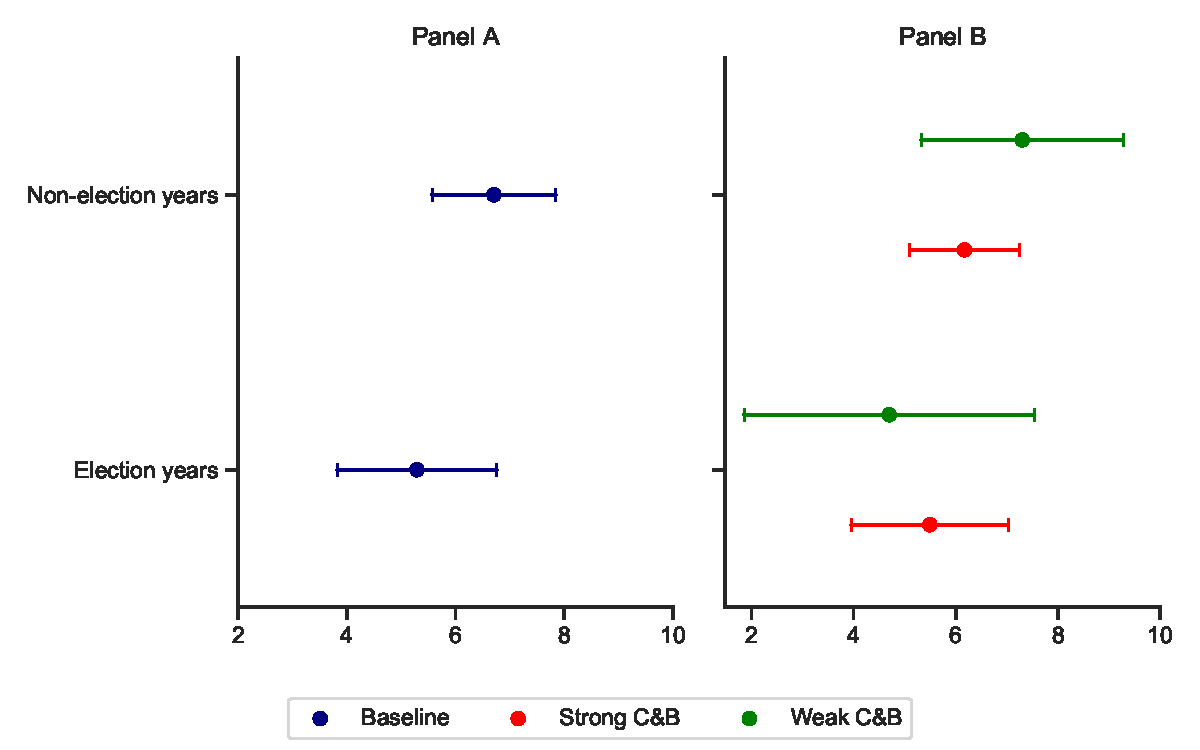
\includegraphics[scale=0.8]{../output/plots/res1.pdf}
	\caption{Unconditional average year-on-year percent change in real household deposit growth rate in election vs. no-election years (Panel A) and the change conditional on the strength of checks and balances on executive power (Panel B). The whiskers represent 95\% confidence intervals, based on the standard errors clustered at the country level.}
	\label{visualresults}
\end{figure}

\begin{figure}[!ht]
	\centering
	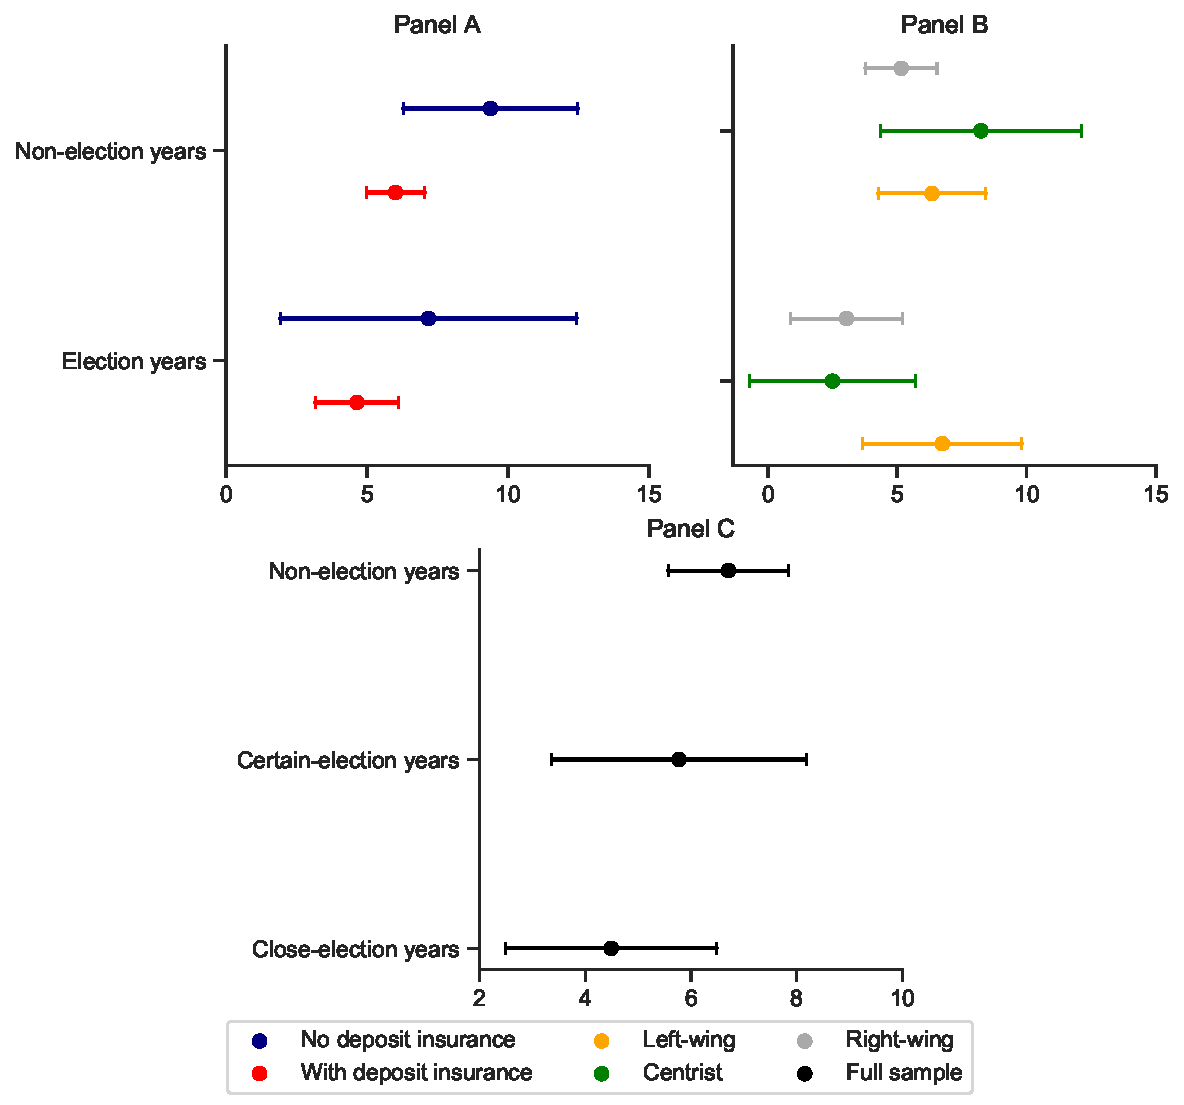
\includegraphics[scale=0.8]{../output/plots/res2.pdf}
	\caption{Average year-on-year percent change in real household deposits outstanding with commercial banks in election vs.\ no-election years conditional on the existence of explicit deposit insurance scheme (Panel A) and conditional on political affiliation of the incumbent state executive (Panel B); average real household deposit growth rates for no-election years, close election years and the election years classified as not close (Panel B). The whiskers represent 95\% confidence intervals, based on the standard errors clustered at the country level.}
	\label{visualresults2}
\end{figure}

In addition, Panel A of Figure \ref{visualresults2} shows that real household deposit growth rates are on average lower  -- during election as well as no-election years -- for the countries that implemented an explicit deposit insurance scheme than for the countries that did not. But it is not clear that the countries that have no explicit deposit insurance scheme experience sharper drops in real household deposit growth during election years than the countries that do have such a scheme -- the difference between the two drops is just about 0.8 p.p. Likewise, Figure \ref{visualresults2}, Panel C seems to reject the hypothesis that closer elections, because they generate more political uncertainty, lead to lower growth in real household deposits: while the average rate for close-election years as well as the rate for the years with ``certain" elections (i.e., the elections not classified as closely contested) is indeed lower than the mean deposit growth for no-election years, there seems to be little difference between the former two rates. On the other hand, Panel B of Figure~\ref{visualresults2} shows that the slide in average real HH deposit growth rates during election years seems to be limited to the elections with right-leaning and centrist incumbents. This result supports my prior conjecture that elections with a market-friendly incumbent generate stronger unease about the potential policy change and therefore lead to larger drops in real HH deposit growth.

I now turn to estimation results for the regressions outlined in Section~\ref{idstrat}. Table~\ref{baselinedeposits} reports the estimates of Equation~\ref{model1}. In Column~(1), I find that the percent change in real household deposits is 1.795 p.p.\ lower relative to no-election years holding macroeconomic business cycle, banking and institutional characteristics constant. Adding time fixed effects in Column~(2), the effect shrinks to -1.625 p.p.; it declines further to -1.475 p.p.\ when we add country fixed effects in Column~(3). These coefficients are statistically significant at 10 percent level and economically meaningful: the election-induced drop in average real household deposit growth represents approximately 25 percent of its sample mean and 16 percent of its standard deviation.\footnote{Hereinafter, I interpret parameters of the models with year and country fixed effects estimated by the within estimator, unless stated otherwise.} Re-estimating Column~(3) with Arellano-Bond difference estimator also yields a negative point estimate for $Election_{it}$, but one that is much smaller in absolute value -- only -0.897. Still, as I have argued in Section~\ref{idstrat} and \hyperlink{appendixA}{Appendix A}, Arellano-Bond estimator is expected to perform poorly in my sample, especially estimating parameters of strictly exogenous variables like $Election_{it}$; thus, Arellano-Bond results should be taken with a grain of salt.


\afterpage{
	{\setstretch{1}
		\begin{longtable}{m{8cm}*{4}{c}}                                         \caption{Political Uncertainty and Bank Deposit Growth: Baseline Results\label{baselinedeposits}}\\                                         \toprule                                         &\multicolumn{4}{c}{$\text{Real HH deposit growth}_{it}$} \\ \cmidrule(lr){2-5}
                    &         (1)   &         (2)   &         (3)   &         (4)   \\
\midrule\endfirsthead                                         \multicolumn{5}{r}{\textit{Table~\ref{baselinedeposits} continued}} \\                                         \toprule\endhead\midrule\endfoot\endlastfoot
$\text{Election}_{it}$&      -1.795*  &      -1.625*  &      -1.475*  &      -0.897   \\
                    &     (0.923)   &     (0.875)   &     (0.842)   &     (0.863)   \\
$\text{Inflation CPI}_{it-1}$&      -0.235** &      -0.245** &      -0.271*  &      -0.010   \\
                    &     (0.099)   &     (0.104)   &     (0.141)   &     (0.173)   \\
$\log(\text{Real GDP per capita}_{it-1})$&      -1.905** &      -1.780** &      -2.038   &     -31.465*  \\
                    &     (0.722)   &     (0.812)   &     (9.518)   &    (16.546)   \\
$\text{Real GDP growth}_{it-1}$&       0.430***&       0.516** &       0.197   &      -0.220   \\
                    &     (0.156)   &     (0.199)   &     (0.209)   &     (0.233)   \\
$\text{Unemployment}_{it-1}$&       0.013   &       0.036   &      -0.215   &      -0.434   \\
                    &     (0.057)   &     (0.058)   &     (0.236)   &     (0.376)   \\
$\text{Capital ratio}_{it-1}$&       0.036   &       0.100   &       0.373   &       0.483   \\
                    &     (0.166)   &     (0.169)   &     (0.427)   &     (1.042)   \\
$\text{Deposits to GDP}_{it-1}$&      -0.006   &      -0.004   &      -0.060   &      -0.072   \\
                    &     (0.007)   &     (0.006)   &     (0.041)   &     (0.079)   \\
$\text{Liquidity ratio}_{it-1}$&       0.052** &       0.043** &       0.077*  &       0.198*  \\
                    &     (0.024)   &     (0.021)   &     (0.042)   &     (0.112)   \\
$\text{Real HH deposit growth}_{it-1}$&       0.076   &       0.033   &      -0.053   &       0.016   \\
                    &     (0.104)   &     (0.105)   &     (0.106)   &     (0.131)   \\
$\text{Property rights}_{it-1}$&      -0.111** &      -0.112** &      -0.149   &      -0.011   \\
                    &     (0.052)   &     (0.050)   &     (0.095)   &     (0.156)   \\
$\text{Corruption perception}_{it-1}$&       0.144** &       0.148** &       0.100   &       0.272   \\
                    &     (0.070)   &     (0.069)   &     (0.130)   &     (0.222)   \\
$\text{Weak C\&B}_{it}$&       0.579   &       0.809   &       0.001   &      -0.634   \\
                    &     (0.713)   &     (0.745)   &     (1.293)   &     (1.857)   \\
\midrule
Observations        &         530   &         530   &         530   &         472   \\
F-test              &       8.484   &       7.729   &       5.130   &       3.068   \\
Estimator           &         OLS   &         OLS   &      Within   &          AB   \\
Year FE             &          No   &         Yes   &         Yes   &         Yes   \\
Country FE          &          No   &          No   &         Yes   &         Yes   \\
N. of instruments   &               &               &               &          38   \\
AR(2) \(p\)         &               &               &               &       0.832   \\
Hansen J test \(p\) &               &               &               &       0.292   \\
\bottomrule                                          \multicolumn{5}{l}{\footnotesize This table presents estimates of the following model:}\\                                          \multicolumn{5}{c}{\footnotesize $ \Delta y_{it} = \beta Election_{it} + X'_{it-1}\kappa +\psi \Delta y_{it-1} + \alpha_i + \alpha_t + \varepsilon_{it}, $}\\                                          \multicolumn{5}{m{\linewidth}}{\footnotesize where $ \Delta y_{it} $ denotes year-on-year percent change in real household deposits with commercial banks in country $ i $ and year $ t $, $ Election_{it} $ is 1 if country $ i $ held an executive election in year $ t $ and $ X_{it-1} $ is the control vector. Standard errors are clustered on the country level and reported in parentheses. Critical values for F-test at 0.01 significance level and actual degrees of freedom range from 2.15 to 2.53. \( * p<0.1, ** p<0.05, *** p<0.01 \).}\\                                          \end{longtable}

		}
}

Estimated coefficients on the control variables suggest that poor countries as well as those with lower inflation and higher real GDP growth enjoy faster real household deposit growth. Among the banking system variables, only the ratio of liquid assets to short-term liabilities seems to have a significant effect at 10 percent level: an increase in the liquidity ratio of 10 percentage points is associated with an increase in real household deposit growth of 0.77 p.p. Furthermore, countries free from corruption maintain higher real deposit growth: going from 25 to 75 percentile seems to add about 3.4 p.p.\ to the country's average real household deposit growth, holding all else constant. Finally, in contrast to the common wisdom that strong property rights boost all kinds of investments, including deposits, my data indicates that stronger property rights correlate with lower real HH deposit growth. This result may be explained by the fact that among investment options available to households (e.g., open a business, invest in a stock market, buy government/private bonds or put money into a deposit account) bank deposits tend to be the safest option, with the difference in risk magnified by weak property rights. For example, if a state does not guarantee proper contract enforcement and/or engages in expropriation of private property, a household is unlikely to open a business, choosing to put their savings into bank deposits instead.

\afterpage{
	{\setstretch{1}
		\begin{longtable}{m{8cm}*{4}{c}}                                         \caption{Political Uncertainty and Bank Deposit Growth: Checks \& Balances \label{cbdeposits}}\\                                         \toprule                                         &\multicolumn{4}{c}{$\text{Real HH deposit growth}_{it}$} \\ \cmidrule(lr){2-5}
                    &         (1)   &         (2)   &         (3)   &         (4)   \\
\midrule\endfirsthead                                         \multicolumn{5}{r}{\textit{Table~\ref{baselinedeposits} continued}} \\                                         \toprule\endhead\midrule\endfoot\endlastfoot
$\text{Election}_{it}$&      -0.764   &      -0.702   &      -0.665   &      -0.104   \\
                    &     (0.848)   &     (0.882)   &     (0.838)   &     (0.854)   \\
$\text{Election}_{it}$ $\times$ $\text{Weak C\&B}_{it}$&      -2.829   &      -2.520   &      -2.204   &      -2.122   \\
                    &     (2.231)   &     (2.332)   &     (2.255)   &     (2.503)   \\
$\text{Weak C\&B}_{it}$&       1.273   &       1.428   &       0.464   &       0.218   \\
                    &     (0.888)   &     (0.934)   &     (1.355)   &     (2.147)   \\
$\text{Property rights}_{it-1}$&      -0.110** &      -0.110** &      -0.148   &      -0.009   \\
                    &     (0.052)   &     (0.050)   &     (0.095)   &     (0.154)   \\
$\text{Corruption perception}_{it-1}$&       0.139*  &       0.143** &       0.095   &       0.273   \\
                    &     (0.070)   &     (0.070)   &     (0.129)   &     (0.219)   \\
$\text{Inflation CPI}_{it-1}$&      -0.235** &      -0.245** &      -0.270*  &       0.001   \\
                    &     (0.099)   &     (0.104)   &     (0.140)   &     (0.172)   \\
$\log(\text{Real GDP per capita}_{it-1})$&      -1.837** &      -1.723** &      -1.783   &     -31.270*  \\
                    &     (0.740)   &     (0.829)   &     (9.371)   &    (16.428)   \\
$\text{Real GDP growth}_{it-1}$&       0.440***&       0.520** &       0.207   &      -0.208   \\
                    &     (0.155)   &     (0.197)   &     (0.206)   &     (0.224)   \\
$\text{Unemployment}_{it-1}$&       0.013   &       0.036   &      -0.217   &      -0.456   \\
                    &     (0.056)   &     (0.057)   &     (0.235)   &     (0.376)   \\
$\text{Capital ratio}_{it-1}$&       0.031   &       0.096   &       0.366   &       0.509   \\
                    &     (0.166)   &     (0.169)   &     (0.425)   &     (1.032)   \\
$\text{Deposits to GDP}_{it-1}$&      -0.006   &      -0.005   &      -0.062   &      -0.074   \\
                    &     (0.007)   &     (0.006)   &     (0.040)   &     (0.078)   \\
$\text{Liquidity ratio}_{it-1}$&       0.053** &       0.044** &       0.077*  &       0.194*  \\
                    &     (0.024)   &     (0.021)   &     (0.042)   &     (0.110)   \\
$\text{Real HH deposit growth}_{it-1}$&       0.075   &       0.033   &      -0.053   &       0.015   \\
                    &     (0.104)   &     (0.105)   &     (0.107)   &     (0.129)   \\
\midrule
Observations        &         530   &         530   &         530   &         472   \\
F-test              &       8.384   &       7.500   &       5.116   &       3.287   \\
Estimator           &         OLS   &         OLS   &      Within   &          AB   \\
Year FE             &          No   &         Yes   &         Yes   &         Yes   \\
Country FE          &          No   &          No   &         Yes   &         Yes   \\
N. of instruments   &               &               &               &          39   \\
AR(2) \(p\)         &               &               &               &       0.788   \\
Hansen J test \(p\) &               &               &               &       0.313   \\
\bottomrule                                          \multicolumn{5}{l}{\footnotesize This table shows estimation results for the following equation:}\\                                          \multicolumn{5}{c}{\footnotesize $ \Delta y_{it} = \beta_1 Election_{it} + \beta_2 Election_{it} \times Weak\ C\&B_{it} + X'_{it-1}\kappa +\psi \Delta y_{it-1} + \alpha_i + \alpha_t + \varepsilon_{it}, $}\\                                          \multicolumn{5}{m{\linewidth}}{\footnotesize where $ \Delta y_{it} $ denotes year-on-year percent change in real household deposits with commercial banks in country $ i $ and year $ t $, $ Election_{it} $ is 1 if country $ i $ held an executive election in year $ t $, $ Weak\ C\&B_{it} $ is 1 if country-year belongs to the bottom half of all country-years with respect to constraints on executive authority and $ X_{it-1} $ is the control vector. Standard errors are clustered on the country level and reported in parentheses. Critical values for F-test at 0.01 significance level and actual degrees of freedom range from 2.17 to 2.48. \( * p<0.1, ** p<0.05, *** p<0.01 \).}\\                                          \end{longtable}

		}
}

Table~\ref{cbdeposits} presents estimated coefficients for Equation~\ref{model2}. The results throughout all specifications suggest that negative effect of the elections on real household deposit growth is concentrated among the country-years with weak checks and balances on executive authority. In particular, the data suggest that the percent change in real household deposits is 2.2 p.p.\ lower in election years for countries with weak constraints on executive power than in election years for countries with strong constraints, ceteris paribus. This difference is economically meaningful, corresponding to 38 percent of the sample mean of real HH deposit growth rate and to 24 percent of its standard deviation. Assuming that elections in the countries with weak checks and balances generate more political uncertainty than elections in the countries with strong checks and balances, the evidence given in Table~\ref{cbdeposits} further affirms my hypothesis that political uncertainty negatively affects real deposit growth. It should be stressed, however, that no causal statements can be made about the parameters of interest $\hat{\beta}_1$ and $\hat{\beta}_2$ since they are not statistically significant.

In Table~\ref{cedeposits}, I report estimation results for Equation~\ref{model3}. Unlike the graphical analysis presented above, Columns~(1)--(3) indicate that close elections are indeed associated with lower real household deposit growth relative to certain elections. The difference between the two is statistically insignificant but large in economic terms: real HH deposit growth is 1.79 p.p.\ lower in close-election years than in certain-election years, which corresponds to 30 percent of this variable's mean and 19 percent of its standard deviation. Simultaneously, the estimate of $\beta_1$ shows that real HH deposit growth in certain-election years is not much different from that in no-election years -- the difference is only 0.58 p.p.\ and again not statistically significant. Taken together, these findings suggest that close elections, which by assumption generate more political uncertainty, are associated with weaker household deposit accumulation. Yet, the lack of statistical significance means that these results should be considered with caution.

\afterpage{
	{\setstretch{1}
		\begin{longtable}{m{8cm}*{4}{c}}                                         \caption{Political Uncertainty and Bank Deposit Growth: Close Elections \label{cedeposits}}\\                                         \toprule                                         &\multicolumn{4}{c}{$\text{Real HH deposit growth}_{it}$} \\ \cmidrule(lr){2-5}
                    &         (1)   &         (2)   &         (3)   &         (4)   \\
\midrule\endfirsthead                                         \multicolumn{5}{r}{\textit{Table~\ref{baselinedeposits} continued}} \\                                         \toprule\endhead\midrule\endfoot\endlastfoot
$\text{Election}_{it}$&      -1.030   &      -0.770   &      -0.583   &      -0.744   \\
                    &     (1.388)   &     (1.305)   &     (1.332)   &     (1.448)   \\
$\text{Close election}_{it}$&      -1.556   &      -1.704   &      -1.790   &      -0.314   \\
                    &     (1.701)   &     (1.598)   &     (1.721)   &     (1.700)   \\
$\text{Property rights}_{it-1}$&      -0.109** &      -0.110** &      -0.143   &      -0.013   \\
                    &     (0.053)   &     (0.051)   &     (0.095)   &     (0.156)   \\
$\text{Corruption perception}_{it-1}$&       0.141*  &       0.144** &       0.107   &       0.273   \\
                    &     (0.070)   &     (0.070)   &     (0.131)   &     (0.222)   \\
$\text{Weak C\&B}_{it}$&       0.531   &       0.754   &       0.038   &      -0.639   \\
                    &     (0.704)   &     (0.733)   &     (1.321)   &     (1.843)   \\
$\text{Inflation CPI}_{it-1}$&      -0.244** &      -0.251** &      -0.271*  &      -0.014   \\
                    &     (0.099)   &     (0.107)   &     (0.140)   &     (0.171)   \\
$\log(\text{Real GDP per capita}_{it-1})$&      -1.900** &      -1.771** &      -2.809   &     -31.444*  \\
                    &     (0.717)   &     (0.808)   &     (9.742)   &    (16.834)   \\
$\text{Real GDP growth}_{it-1}$&       0.418** &       0.502** &       0.189   &      -0.219   \\
                    &     (0.158)   &     (0.202)   &     (0.208)   &     (0.234)   \\
$\text{Unemployment}_{it-1}$&       0.007   &       0.030   &      -0.226   &      -0.432   \\
                    &     (0.058)   &     (0.059)   &     (0.234)   &     (0.378)   \\
$\text{Capital ratio}_{it-1}$&       0.033   &       0.096   &       0.362   &       0.475   \\
                    &     (0.168)   &     (0.172)   &     (0.430)   &     (1.054)   \\
$\text{Deposits to GDP}_{it-1}$&      -0.007   &      -0.005   &      -0.064   &      -0.073   \\
                    &     (0.007)   &     (0.006)   &     (0.041)   &     (0.080)   \\
$\text{Liquidity ratio}_{it-1}$&       0.053** &       0.043** &       0.075*  &       0.198*  \\
                    &     (0.024)   &     (0.021)   &     (0.041)   &     (0.112)   \\
$\text{Real HH deposit growth}_{it-1}$&       0.077   &       0.035   &      -0.051   &       0.015   \\
                    &     (0.104)   &     (0.106)   &     (0.107)   &     (0.132)   \\
\midrule
Observations        &         530   &         530   &         530   &         472   \\
F-test              &       7.846   &       7.159   &       5.852   &       3.050   \\
Estimator           &         OLS   &         OLS   &      Within   &          AB   \\
Year FE             &          No   &         Yes   &         Yes   &         Yes   \\
Country FE          &          No   &          No   &         Yes   &         Yes   \\
N. of instruments   &               &               &               &          39   \\
AR(2) \(p\)         &               &               &               &       0.824   \\
Hansen J test \(p\) &               &               &               &       0.291   \\
\bottomrule                                          \multicolumn{5}{l}{\footnotesize This table shows estimates for the following model:}\\                                          \multicolumn{5}{c}{\footnotesize $ \Delta y_{it} = \beta_1 Election_{it} + \beta_2 Close\ Election_{it} + X'_{it-1}\kappa +\psi \Delta y_{it-1} + \alpha_i + \alpha_t + \varepsilon_{it}, $}\\                                          \multicolumn{5}{m{\linewidth}}{\footnotesize where $ \Delta y_{it} $ denotes year-on-year percent change in real household deposits with commercial banks in country $ i $ and year $ t $, $ Election_{it} $ is 1 if country $ i $ held an executive election in year $ t $, $ Close\ Election_{it} $ is 1 if margin of victory in the relevant election belongs to the bottom 50 percentile. $ X_{it-1} $ is the control vector. Standard errors are clustered on the country level and reported in parentheses. Critical values for F-test at 0.01 significance level and actual degrees of freedom range from 2.13 to 2.48. \( * p<0.1, ** p<0.05, *** p<0.01 \).}\\                                          \end{longtable}

		\clearpage
		\begin{longtable}{m{8cm}*{4}{c}}                                         \caption{Political Uncertainty and Bank Deposit Growth: Political Affiliation of the Incumbent \label{rldeposits}}\\                                         \toprule                                         &\multicolumn{4}{c}{$\text{Real HH deposit growth}_{it}$} \\ \cmidrule(lr){2-5}
                    &         (1)   &         (2)   &         (3)   &         (4)   \\
\midrule\endfirsthead                                         \multicolumn{5}{r}{\textit{Table~\ref{baselinedeposits} continued}} \\                                         \toprule\endhead\midrule\endfoot\endlastfoot
$\text{Election}_{it}$&       0.942   &       1.362   &       1.202   &       1.422   \\
                    &     (2.147)   &     (2.138)   &     (2.138)   &     (2.250)   \\
$\text{Election}_{it}$ $\times$ $\text{Market-friendly}_{it}$&      -4.684** &      -5.178** &      -4.826*  &      -4.438   \\
                    &     (2.238)   &     (2.313)   &     (2.418)   &     (2.768)   \\
$\text{Market-friendly}_{it}$&      -0.064   &       0.276   &       1.969   &       1.596   \\
                    &     (1.230)   &     (1.282)   &     (1.861)   &     (2.002)   \\
$\text{Property rights}_{it-1}$&      -0.145** &      -0.148** &      -0.070   &       0.184   \\
                    &     (0.068)   &     (0.066)   &     (0.124)   &     (0.229)   \\
$\text{Corruption perception}_{it-1}$&       0.196** &       0.202** &       0.180   &       0.241   \\
                    &     (0.088)   &     (0.084)   &     (0.143)   &     (0.273)   \\
$\text{Weak C\&B}_{it}$&       0.284   &       0.576   &       0.220   &      -0.818   \\
                    &     (0.956)   &     (0.954)   &     (1.506)   &     (2.310)   \\
$\text{Inflation CPI}_{it-1}$&      -0.357*  &      -0.356   &      -0.276   &      -0.098   \\
                    &     (0.203)   &     (0.216)   &     (0.323)   &     (0.313)   \\
$\log(\text{Real GDP per capita}_{it-1})$&      -2.357***&      -2.179** &      -3.231   &     -14.324   \\
                    &     (0.869)   &     (0.998)   &    (15.099)   &    (23.732)   \\
$\text{Real GDP growth}_{it-1}$&       0.575** &       0.697*  &       0.202   &      -0.373   \\
                    &     (0.249)   &     (0.354)   &     (0.395)   &     (0.343)   \\
$\text{Unemployment}_{it-1}$&       0.007   &       0.038   &      -0.277   &      -0.121   \\
                    &     (0.084)   &     (0.084)   &     (0.288)   &     (0.521)   \\
$\text{Capital ratio}_{it-1}$&      -0.080   &      -0.018   &      -0.210   &      -0.613   \\
                    &     (0.198)   &     (0.193)   &     (0.358)   &     (1.530)   \\
$\text{Deposits to GDP}_{it-1}$&      -0.002   &      -0.001   &      -0.041   &      -0.159   \\
                    &     (0.007)   &     (0.006)   &     (0.041)   &     (0.145)   \\
$\text{Liquidity ratio}_{it-1}$&       0.048*  &       0.043*  &       0.038   &       0.183   \\
                    &     (0.026)   &     (0.024)   &     (0.042)   &     (0.112)   \\
$\text{Real HH deposit growth}_{it-1}$&      -0.033   &      -0.063   &      -0.160   &      -0.060   \\
                    &     (0.119)   &     (0.122)   &     (0.123)   &     (0.162)   \\
\midrule
Observations        &         392   &         392   &         392   &         340   \\
F-test              &       7.299   &       8.434   &       5.895   &       4.605   \\
Estimator           &         OLS   &         OLS   &      Within   &          AB   \\
Year FE             &          No   &         Yes   &         Yes   &         Yes   \\
Country FE          &          No   &          No   &         Yes   &         Yes   \\
N. of instruments   &               &               &               &          36   \\
AR(2) \(p\)         &               &               &               &       0.564   \\
Hansen J test \(p\) &               &               &               &       0.119   \\
\bottomrule                                          \multicolumn{5}{l}{\footnotesize This table presents estimation results for the following equation:}\\                                          \multicolumn{5}{c}{\footnotesize $ \Delta y_{it} = \beta_1 Election_{it} + \beta_2 Election_{it} \times MF_{it} + \beta_3 MF_{it} + X'_{it-1}\kappa +\psi \Delta y_{it-1} + \alpha_i + \alpha_t + \varepsilon_{it}, $}\\                                          \multicolumn{5}{m{\linewidth}}{\footnotesize where $ \Delta y_{it} $ denotes year-on-year percent change in real household deposits with commercial banks in country $ i $ and year $ t $, $ Election_{it} $ is 1 if country $ i $ held an executive election in year $ t $, $ MF_{it} $ is 1 if the incumbent is right- or center-leaning and $ X_{it-1} $ is the control vector. Standard errors are clustered on the country level and reported in parentheses. Critical values for F-test at 0.01 significance level and actual degrees of freedom range from 2.18 to 2.50. \( * p<0.1, ** p<0.05, *** p<0.01 \).}\\                                          \end{longtable}

		\clearpage
		\begin{longtable}{m{8cm}*{4}{c}}                                         \caption{Political Uncertainty and Bank Deposit Growth: Deposit Insurance \label{dideposits}}\\                                         \toprule                                         &\multicolumn{4}{c}{$\text{Real HH deposit growth}_{it}$} \\ \cmidrule(lr){2-5}
                    &         (1)   &         (2)   &         (3)   &         (4)   \\
\midrule\endfirsthead                                         \multicolumn{5}{r}{\textit{Table~\ref{baselinedeposits} continued}} \\                                         \toprule\endhead\midrule\endfoot\endlastfoot
$\text{Election}_{it}$&      -2.163   &      -1.242   &      -0.732   &      -0.206   \\
                    &     (4.749)   &     (4.707)   &     (4.582)   &     (5.943)   \\
$\text{Election}_{it}$ $\times$ $\text{Deposit insurance}_{it-1}$&       0.405   &      -0.364   &      -0.853   &      -1.345   \\
                    &     (4.779)   &     (4.789)   &     (4.703)   &     (6.027)   \\
$\text{Deposit insurance}_{it-1}$&      -1.652   &      -1.455   &       1.616   &     -10.967** \\
                    &     (2.100)   &     (2.115)   &     (1.992)   &     (4.644)   \\
$\text{Property rights}_{it-1}$&      -0.092** &      -0.090** &      -0.133   &       0.041   \\
                    &     (0.041)   &     (0.040)   &     (0.100)   &     (0.188)   \\
$\text{Corruption perception}_{it-1}$&       0.103*  &       0.102*  &       0.067   &       0.126   \\
                    &     (0.054)   &     (0.056)   &     (0.152)   &     (0.254)   \\
$\text{Weak C\&B}_{it}$&       0.152   &       0.431   &       0.417   &       1.137   \\
                    &     (0.717)   &     (0.761)   &     (1.558)   &     (2.512)   \\
$\text{Inflation CPI}_{it-1}$&      -0.351** &      -0.376** &      -0.371   &       0.001   \\
                    &     (0.160)   &     (0.179)   &     (0.232)   &     (0.277)   \\
$\log(\text{Real GDP per capita}_{it-1})$&      -2.024***&      -1.965** &      -8.657   &     -48.661** \\
                    &     (0.703)   &     (0.807)   &    (13.619)   &    (23.831)   \\
$\text{Real GDP growth}_{it-1}$&       0.360** &       0.371*  &       0.176   &      -0.232   \\
                    &     (0.160)   &     (0.214)   &     (0.249)   &     (0.282)   \\
$\text{Unemployment}_{it-1}$&       0.011   &       0.032   &      -0.298   &      -0.890** \\
                    &     (0.076)   &     (0.079)   &     (0.267)   &     (0.426)   \\
$\text{Capital ratio}_{it-1}$&       0.003   &       0.072   &       0.068   &      -2.406   \\
                    &     (0.179)   &     (0.180)   &     (0.486)   &     (2.366)   \\
$\text{Deposits to GDP}_{it-1}$&      -0.006   &      -0.003   &      -0.038   &       0.051   \\
                    &     (0.007)   &     (0.006)   &     (0.038)   &     (0.066)   \\
$\text{Liquidity ratio}_{it-1}$&       0.070***&       0.062***&       0.068   &       0.306   \\
                    &     (0.026)   &     (0.022)   &     (0.050)   &     (0.192)   \\
$\text{Real HH deposit growth}_{it-1}$&       0.062   &       0.020   &      -0.073   &       0.012   \\
                    &     (0.098)   &     (0.098)   &     (0.100)   &     (0.124)   \\
\midrule
Observations        &         436   &         436   &         436   &         378   \\
F-test              &       8.507   &       7.567   &       2.459   &      19.631   \\
Estimator           &         OLS   &         OLS   &      Within   &          AB   \\
Year FE             &          No   &         Yes   &         Yes   &         Yes   \\
Country FE          &          No   &          No   &         Yes   &         Yes   \\
N. of instruments   &               &               &               &          34   \\
AR(2) \(p\)         &               &               &               &       0.590   \\
Hansen J test \(p\) &               &               &               &       0.094   \\
\bottomrule                                          \multicolumn{5}{l}{\footnotesize This table reports estimation results for the following model:}\\                                          \multicolumn{5}{c}{\footnotesize $ \Delta y_{it} = \beta_1 Election_{it} + \beta_2 Election_{it} \times DI_{it-1} + \beta_3 DI_{it-1} + X'_{it-1}\kappa + \psi \Delta y_{it-1} + \alpha_i + \alpha_t + \varepsilon_{it}, $}\\                                          \multicolumn{5}{m{\linewidth}}{\footnotesize where $ \Delta y_{it} $ denotes year-on-year percent change in real household deposits with commercial banks in country $ i $ and year $ t $, $ Election_{it} $ is 1 if country $ i $ held an executive election in year $ t $, $ DI_{it-1} $ is 1 if country $ i $ has explicit deposit insurance scheme in year $ t-1 $, $ X_{it-1} $ is the control vector. Standard errors are clustered on the country level and reported in parentheses. Critical values for F-test at 0.01 significance level and actual degrees of freedom range from 2.11 to 2.46. \( * p<0.1, ** p<0.05, *** p<0.01 \).}\\                                          \end{longtable}

		}
}

Table~\ref{rldeposits} shows estimation results for Equation~\ref{model4}. I find that the elections with a market-friendly incumbent -- i.e., a right-leaning or centrist one -- are associated with a statistically significant (at 10 percent level) drop of 4.83 p.p.\ in real household deposit growth relative to the election years when a left-leaning executive was in power, holding all else equal. This effect remains broadly constant across all specifications; it is also huge in economic terms, corresponding to 83 percent of real HH deposit growth's mean and 53 percent of its standard deviation. Furthermore, the estimates suggest that depositors welcome a potential change away from leftist policies, since real household deposit growth in election years with a leftist incumbent is about 1.2 p.p.\ higher relative to the no-election years -- although, admittedly, $\hat{\beta}_1$ is not statistically different from 0 in all columns of Table~\ref{rldeposits}.

Finally, estimation results for Equation~\eqref{model5}, reported in Table~\ref{dideposits}, are mixed: Column~(1) reports a positive $\hat{\beta}_2$, while Columns~(2)--(4) report a negative one. The estimated parameter of interest is neither statistically significant, nor large in magnitude, apart from the results in Column~(4), indicating that the existence of an explicit deposit insurance scheme is not a particularly important determinant of depositor behavior. Combined with the results in Tables~\ref{baselinedeposits}--\ref{rldeposits}, this finding suggests that political uncertainty affects real household deposits through other factors that have an impact on their net present value and that a post-election government can influence -- such as inflation and currency exchange rate -- rather than through changing the probability of bank default.

Taken together, the findings presented in this section are in line with the hypotheses outlined in Section~\ref{idstrat}, suggesting that political uncertainty is indeed associated with lower real household deposit growth.

\section{Political Uncertainty and Bank Lending}\label{lendingresults}
Next, I explore if this negative shock to bank deposits induced by political uncertainty is transmitted to bank lending. The models estimated in this section are identical to the ones in Equations~\eqref{model1}--\eqref{model4}, except for a modified banking-system control vector $B_{it-1}$. As in the previous sections, I use capital to assets ratio and liquid assets to short-term liabilities to account for the effects of bank capitalization and liquidity on lending. I supplement these variables with bank credit to deposits ratio to control for the possibility that banks may be unable or less eager to extend additional loans when they have lent lavishly already. I also control for banking system concentration -- measured as a share of 3 largest banks' assets in total assets of the commercial banking system -- since some studies suggest that it may have negative influence on banks' lending \citep[see, for example,][]{beck2004bank, braggion2017nothing}. All these regressors are taken from the GFDD and lagged one year. The dependent variable is year-on-year percent change in real outstanding loans with commercial banks winsorized at 1 percent level (hereafter also referred to as real loan growth or real lending growth). Note that Equation~\eqref{model5} is not estimated in this section, for I do not find any sizable effect of explicit deposit insurance on the relationship between elections and real household deposit growth in Section~\ref{mainresults}.

\afterpage{
	{\setstretch{1}
		\begin{longtable}{m{8cm}*{4}{c}}                                         \caption{Political Uncertainty and Bank Loan Growth: Baseline Results \label{baselineloans}}\\                                         \toprule                                         &\multicolumn{4}{c}{$\text{Real loan growth}_{it}$} \\ \cmidrule(lr){2-5}
                    &         (1)   &         (2)   &         (3)   &         (4)   \\
\midrule\endfirsthead                                         \multicolumn{5}{r}{\textit{Table~\ref{baselineloans} continued}} \\                                         \toprule\endhead\midrule\endfoot\endlastfoot
$\text{Election}_{it}$&      -0.655   &      -0.445   &      -0.428   &      -0.204   \\
                    &     (0.945)   &     (0.849)   &     (0.829)   &     (0.956)   \\
$\text{Inflation CPI}_{it-1}$&      -0.230** &      -0.139** &      -0.277***&      -0.057   \\
                    &     (0.091)   &     (0.070)   &     (0.094)   &     (0.173)   \\
$\log(\text{Real GDP per capita}_{it-1})$&      -0.866** &      -0.632   &      -6.097   &     -23.237   \\
                    &     (0.395)   &     (0.397)   &     (6.616)   &    (16.388)   \\
$\text{Real GDP growth}_{it-1}$&       0.400***&       0.515***&       0.407***&      -0.095   \\
                    &     (0.126)   &     (0.134)   &     (0.154)   &     (0.182)   \\
$\text{Unemployment}_{it-1}$&      -0.031   &      -0.027   &      -0.436** &      -0.326   \\
                    &     (0.046)   &     (0.049)   &     (0.206)   &     (0.355)   \\
$\text{Capital ratio}_{it-1}$&       0.004   &       0.056   &      -0.279   &       1.355   \\
                    &     (0.130)   &     (0.126)   &     (0.385)   &     (1.037)   \\
$\text{Credit to deposits}_{it-1}$&      -0.014** &      -0.014** &      -0.067*  &       0.005   \\
                    &     (0.007)   &     (0.006)   &     (0.037)   &     (0.082)   \\
$\text{Bank concentration}_{it-1}$&       0.009   &       0.007   &       0.061   &       0.235   \\
                    &     (0.017)   &     (0.016)   &     (0.063)   &     (0.275)   \\
$\text{Liquidity ratio}_{it-1}$&       0.068***&       0.054** &       0.078   &       0.279*  \\
                    &     (0.023)   &     (0.020)   &     (0.058)   &     (0.143)   \\
$\text{Real loan growth}_{it-1}$&       0.434***&       0.378***&       0.279***&       0.362***\\
                    &     (0.058)   &     (0.058)   &     (0.064)   &     (0.093)   \\
$\text{Property rights}_{it-1}$&      -0.034   &      -0.049   &      -0.216** &      -0.290*  \\
                    &     (0.031)   &     (0.032)   &     (0.088)   &     (0.149)   \\
$\text{Corruption perception}_{it-1}$&      -0.015   &       0.003   &      -0.125   &      -0.141   \\
                    &     (0.038)   &     (0.037)   &     (0.112)   &     (0.169)   \\
$\text{Weak C\&B}_{it}$&      -0.192   &      -0.139   &      -0.861   &       0.397   \\
                    &     (0.549)   &     (0.520)   &     (0.935)   &     (1.311)   \\
\midrule
Observations        &         744   &         744   &         744   &         662   \\
F-test              &      59.770   &      62.834   &      30.931   &      12.743   \\
Estimator           &         OLS   &         OLS   &      Within   &          AB   \\
Year FE             &          No   &         Yes   &         Yes   &         Yes   \\
Country FE          &          No   &          No   &         Yes   &         Yes   \\
N. of instruments   &               &               &               &          43   \\
AR(2) \(p\)         &               &               &               &       0.125   \\
Hansen J test \(p\) &               &               &               &       0.039   \\
\bottomrule                                          \multicolumn{5}{l}{\footnotesize This table presents estimates of the following model:}\\                                          \multicolumn{5}{c}{\footnotesize $ \Delta y_{it} = \beta Election_{it} + X'_{it-1}\kappa +\psi \Delta y_{it-1} + \alpha_i + \alpha_t + \varepsilon_{it}, $}\\                                          \multicolumn{5}{m{\linewidth}}{\footnotesize where $ \Delta y_{it} $ denotes year-on-year percent change in real loans outstanding with commercial banks in country $ i $ and year $ t $, $ Election_{it} $ is 1 if country $ i $ held an executive election in year $ t $ and $ X_{it-1} $ is the control vector. Standard errors are clustered on the country level and reported in parentheses. Critical values for F-test at 0.01 significance level and actual degrees of freedom range from 2.02 to 2.38. \( * p<0.1, ** p<0.05, *** p<0.01 \).}\\                                          \end{longtable}

		\clearpage
		\begin{longtable}{m{8cm}*{4}{c}}                                         \caption{Political Uncertainty and Bank Loan Growth: Checks \& Balances \label{cbloans}}\\                                         \toprule                                         &\multicolumn{4}{c}{$\text{Real loan growth}_{it}$} \\ \cmidrule(lr){2-5}
                    &         (1)   &         (2)   &         (3)   &         (4)   \\
\midrule\endfirsthead                                         \multicolumn{5}{r}{\textit{Table~\ref{cbloans} continued}} \\                                         \toprule\endhead\midrule\endfoot\endlastfoot
$\text{Election}_{it}$&      -2.092** &      -2.284***&      -2.358***&      -1.891*  \\
                    &     (0.995)   &     (0.836)   &     (0.833)   &     (1.045)   \\
$\text{Election}_{it}$ $\times$ $\text{Weak C\&B}_{it}$&       3.358*  &       4.285** &       4.475** &       3.951*  \\
                    &     (1.893)   &     (1.784)   &     (1.790)   &     (2.234)   \\
$\text{Weak C\&B}_{it}$&      -0.998   &      -1.165   &      -1.828*  &      -1.136   \\
                    &     (0.739)   &     (0.710)   &     (1.012)   &     (1.359)   \\
$\text{Property rights}_{it-1}$&      -0.037   &      -0.054   &      -0.220** &      -0.299** \\
                    &     (0.032)   &     (0.033)   &     (0.090)   &     (0.149)   \\
$\text{Corruption perception}_{it-1}$&      -0.008   &       0.012   &      -0.115   &      -0.136   \\
                    &     (0.039)   &     (0.038)   &     (0.112)   &     (0.173)   \\
$\text{Inflation CPI}_{it-1}$&      -0.230** &      -0.140** &      -0.278***&      -0.054   \\
                    &     (0.090)   &     (0.070)   &     (0.091)   &     (0.175)   \\
$\log(\text{Real GDP per capita}_{it-1})$&      -0.902** &      -0.675*  &      -6.530   &     -22.378   \\
                    &     (0.391)   &     (0.391)   &     (6.568)   &    (16.475)   \\
$\text{Real GDP growth}_{it-1}$&       0.395***&       0.508***&       0.386** &      -0.122   \\
                    &     (0.123)   &     (0.129)   &     (0.148)   &     (0.185)   \\
$\text{Unemployment}_{it-1}$&      -0.029   &      -0.024   &      -0.436** &      -0.260   \\
                    &     (0.047)   &     (0.049)   &     (0.205)   &     (0.347)   \\
$\text{Capital ratio}_{it-1}$&       0.010   &       0.066   &      -0.243   &       1.357   \\
                    &     (0.128)   &     (0.124)   &     (0.382)   &     (1.041)   \\
$\text{Credit to deposits}_{it-1}$&      -0.015** &      -0.015** &      -0.066*  &       0.006   \\
                    &     (0.007)   &     (0.006)   &     (0.037)   &     (0.082)   \\
$\text{Bank concentration}_{it-1}$&       0.009   &       0.008   &       0.063   &       0.205   \\
                    &     (0.016)   &     (0.016)   &     (0.062)   &     (0.274)   \\
$\text{Liquidity ratio}_{it-1}$&       0.067***&       0.052** &       0.080   &       0.279*  \\
                    &     (0.023)   &     (0.020)   &     (0.057)   &     (0.140)   \\
$\text{Real loan growth}_{it-1}$&       0.435***&       0.379***&       0.281***&       0.368***\\
                    &     (0.057)   &     (0.057)   &     (0.063)   &     (0.092)   \\
\midrule
Observations        &         744   &         744   &         744   &         662   \\
F-test              &      60.051   &      67.575   &      38.930   &      14.211   \\
Estimator           &         OLS   &         OLS   &      Within   &          AB   \\
Year FE             &          No   &         Yes   &         Yes   &         Yes   \\
Country FE          &          No   &          No   &         Yes   &         Yes   \\
N. of instruments   &               &               &               &          44   \\
AR(2) \(p\)         &               &               &               &       0.137   \\
Hansen J test \(p\) &               &               &               &       0.025   \\
\bottomrule                                          \multicolumn{5}{l}{\footnotesize This table shows estimation results for the following equation:}\\                                          \multicolumn{5}{c}{\footnotesize $ \Delta y_{it} = \beta_1 Election_{it} + \beta_2 Election_{it} \times Weak\ C\&B_{it} + X'_{it-1}\kappa +\psi \Delta y_{it-1} + \alpha_i + \alpha_t + \varepsilon_{it}, $}\\                                          \multicolumn{5}{m{\linewidth}}{\footnotesize where $ \Delta y_{it} $ denotes year-on-year percent change in real loans with commercial banks in country $ i $ and year $ t $, $ Election_{it} $ is 1 if country $ i $ held an executive election in year $ t $, $ Weak\ C\&B_{it} $ is 1 if country-year belongs to the bottom half of all country-years with respect to constraints on executive authority and $ X_{it-1} $ is the control vector. Standard errors are clustered on the country level and reported in parentheses. Critical values for F-test at 0.01 significance level and actual degrees of freedom range from 2.01 to 2.33. \( * p<0.1, ** p<0.05, *** p<0.01 \).}\\                                          \end{longtable}

	}
}

Table~\ref{baselineloans} reports estimates of the bank lending regression \`a la Equation~\eqref{model1}. $\hat{\beta}$ is negative but very small and not statistically significant, ranging from -0.66 to -0.2 depending on the specification. As for the control variables, the results suggest that real loan growth is negatively associated with inflation and credit to deposits ratio, and positively -- with real GDP growth rate, liquidity ratio and its own 1-year lag, all else equal.

The results of estimating Equation~\eqref{model2} with real loan growth as the dependent variable are presented in Table~\ref{cbloans}. I find a negative and statistically significant association between elections and real loan growth for the countries with strong checks and balances on their executive authority: this group endures 2.36 p.p.\ lower year-on-year percent change in real loans outstanding in election years than in no-election years, ceteris paribus. This effect constitutes 35 percent of the average real loan growth and 21 percent of this variable's standard deviation. In contrast with my findings on deposits, $\hat{\beta}_2$ is positive: real loan growth during election years for the countries with weak C\&B is 4.48 p.p.\ higher relative to the election years for the strong-C\&B countries -- an effect that is both statistically significant at 5 percent level and economically large. These estimates do not favor the hypothesis that banks transmit political-uncertainty-induced deposit shock to bank lending. But they are consistent with findings of \citet{dincc2005politicians} and others who document that the incumbent politicians tend to pressure banks to extend more loans around elections in order to improve their electoral chances: the weaker the constraints on the executive authority are, the more levers the incumbent has to influence banks' lending decisions which, in turn, leads to higher lending growth rates around elections for the weak-C\&B countries.

\afterpage{
	{\setstretch{1}
		\begin{longtable}{m{8cm}*{4}{c}}                                         \caption{Political Uncertainty and Bank Loan Growth: Close Elections \label{celoans}}\\                                         \toprule                                         &\multicolumn{4}{c}{$\text{Real loan growth}_{it}$} \\ \cmidrule(lr){2-5}
                    &         (1)   &         (2)   &         (3)   &         (4)   \\
\midrule\endfirsthead                                         \multicolumn{5}{r}{\textit{Table~\ref{celoans} continued}} \\                                         \toprule\endhead\midrule\endfoot\endlastfoot
$\text{Election}_{it}$&       0.423   &       1.072   &       1.240   &       1.933   \\
                    &     (1.318)   &     (1.220)   &     (1.278)   &     (1.361)   \\
$\text{Close election}_{it}$&      -2.151   &      -2.987** &      -3.323** &      -4.354** \\
                    &     (1.617)   &     (1.424)   &     (1.581)   &     (1.742)   \\
$\text{Property rights}_{it-1}$&      -0.029   &      -0.043   &      -0.205** &      -0.308** \\
                    &     (0.031)   &     (0.031)   &     (0.089)   &     (0.154)   \\
$\text{Corruption perception}_{it-1}$&      -0.020   &      -0.005   &      -0.121   &      -0.140   \\
                    &     (0.038)   &     (0.037)   &     (0.112)   &     (0.167)   \\
$\text{Weak C\&B}_{it}$&      -0.239   &      -0.208   &      -0.813   &       0.612   \\
                    &     (0.553)   &     (0.527)   &     (0.983)   &     (1.390)   \\
$\text{Inflation CPI}_{it-1}$&      -0.236** &      -0.144** &      -0.279***&      -0.076   \\
                    &     (0.093)   &     (0.069)   &     (0.092)   &     (0.174)   \\
$\log(\text{Real GDP per capita}_{it-1})$&      -0.876** &      -0.640   &      -7.126   &     -25.022   \\
                    &     (0.396)   &     (0.400)   &     (6.530)   &    (16.821)   \\
$\text{Real GDP growth}_{it-1}$&       0.389***&       0.500***&       0.400***&      -0.112   \\
                    &     (0.123)   &     (0.129)   &     (0.151)   &     (0.183)   \\
$\text{Unemployment}_{it-1}$&      -0.037   &      -0.035   &      -0.458** &      -0.411   \\
                    &     (0.046)   &     (0.049)   &     (0.201)   &     (0.361)   \\
$\text{Capital ratio}_{it-1}$&       0.009   &       0.061   &      -0.262   &       1.289   \\
                    &     (0.130)   &     (0.126)   &     (0.386)   &     (1.097)   \\
$\text{Credit to deposits}_{it-1}$&      -0.014** &      -0.014** &      -0.066*  &       0.006   \\
                    &     (0.007)   &     (0.006)   &     (0.037)   &     (0.081)   \\
$\text{Bank concentration}_{it-1}$&       0.008   &       0.006   &       0.062   &       0.247   \\
                    &     (0.017)   &     (0.016)   &     (0.065)   &     (0.270)   \\
$\text{Liquidity ratio}_{it-1}$&       0.069***&       0.055***&       0.075   &       0.273*  \\
                    &     (0.023)   &     (0.020)   &     (0.057)   &     (0.141)   \\
$\text{Real loan growth}_{it-1}$&       0.435***&       0.381***&       0.282***&       0.363***\\
                    &     (0.057)   &     (0.057)   &     (0.063)   &     (0.094)   \\
\midrule
Observations        &         744   &         744   &         744   &         662   \\
F-test              &      55.470   &      58.888   &      34.882   &      13.316   \\
Estimator           &         OLS   &         OLS   &      Within   &          AB   \\
Year FE             &          No   &         Yes   &         Yes   &         Yes   \\
Country FE          &          No   &          No   &         Yes   &         Yes   \\
N. of instruments   &               &               &               &          44   \\
AR(2) \(p\)         &               &               &               &       0.095   \\
Hansen J test \(p\) &               &               &               &       0.041   \\
\bottomrule                                          \multicolumn{5}{l}{\footnotesize This table shows estimates for the following model:}\\                                          \multicolumn{5}{c}{\footnotesize $ \Delta y_{it} = \beta_1 Election_{it} + \beta_2 Close\ Election_{it} + X'_{it-1}\kappa +\psi \Delta y_{it-1} + \alpha_i + \alpha_t + \varepsilon_{it}, $}\\                                          \multicolumn{5}{m{\linewidth}}{\footnotesize where $ \Delta y_{it} $ denotes year-on-year percent change in real loans with commercial banks in country $ i $ and year $ t $, $ Election_{it} $ is 1 if country $ i $ held an executive election in year $ t $, $ Close\ Election_{it} $ is 1 if margin of victory in the relevant election belongs to the bottom 50 percentile. $ X_{it-1} $ is the control vector. Standard errors are clustered on the country level and reported in parentheses. Critical values for F-test at 0.01 significance level and actual degrees of freedom range from 2.01 to 2.33. \( * p<0.1, ** p<0.05, *** p<0.01 \).}\\                                          \end{longtable}

		\clearpage
		\begin{longtable}{m{8cm}*{4}{c}}                                         \caption{Political Uncertainty and Bank Loan Growth: Incumbent's Affiliation\label{rlloans}}\\                                         \toprule                                         &\multicolumn{4}{c}{$\text{Real loan growth}_{it}$} \\ \cmidrule(lr){2-5}
                    &         (1)   &         (2)   &         (3)   &         (4)   \\
\midrule\endfirsthead                                         \multicolumn{5}{r}{\textit{Table~\ref{rlloans} continued}} \\                                         \toprule\endhead\midrule\endfoot\endlastfoot
$\text{Election}_{it}$&       1.229   &       2.074   &       1.855   &       1.920   \\
                    &     (2.196)   &     (2.052)   &     (2.116)   &     (2.676)   \\
$\text{Election}_{it}$ $\times$ $\text{Market-friendly}_{it}$&      -2.644   &      -3.614*  &      -3.658   &      -3.793   \\
                    &     (2.285)   &     (2.143)   &     (2.299)   &     (2.912)   \\
$\text{Market-friendly}_{it}$&      -0.159   &      -0.205   &       1.188   &       2.961   \\
                    &     (0.815)   &     (0.810)   &     (1.311)   &     (2.416)   \\
$\text{Property rights}_{it-1}$&      -0.047   &      -0.068*  &      -0.244*  &      -0.238   \\
                    &     (0.039)   &     (0.037)   &     (0.124)   &     (0.181)   \\
$\text{Corruption perception}_{it-1}$&      -0.020   &       0.000   &      -0.068   &      -0.161   \\
                    &     (0.044)   &     (0.042)   &     (0.117)   &     (0.194)   \\
$\text{Weak C\&B}_{it}$&      -1.181   &      -1.036   &      -1.468   &       0.478   \\
                    &     (0.719)   &     (0.677)   &     (1.126)   &     (1.496)   \\
$\text{Inflation CPI}_{it-1}$&      -0.281** &      -0.214** &      -0.393** &      -0.051   \\
                    &     (0.131)   &     (0.102)   &     (0.156)   &     (0.177)   \\
$\log(\text{Real GDP per capita}_{it-1})$&      -0.999*  &      -0.800   &      -4.017   &     -11.718   \\
                    &     (0.506)   &     (0.538)   &     (7.987)   &    (20.906)   \\
$\text{Real GDP growth}_{it-1}$&       0.548***&       0.634***&       0.440** &      -0.064   \\
                    &     (0.163)   &     (0.181)   &     (0.168)   &     (0.242)   \\
$\text{Unemployment}_{it-1}$&      -0.028   &      -0.035   &      -0.643***&      -0.581   \\
                    &     (0.076)   &     (0.075)   &     (0.233)   &     (0.568)   \\
$\text{Capital ratio}_{it-1}$&      -0.175   &      -0.107   &      -0.525   &      -0.030   \\
                    &     (0.120)   &     (0.116)   &     (0.364)   &     (1.542)   \\
$\text{Credit to deposits}_{it-1}$&      -0.012*  &      -0.013** &      -0.058   &      -0.067   \\
                    &     (0.007)   &     (0.006)   &     (0.037)   &     (0.096)   \\
$\text{Bank concentration}_{it-1}$&       0.007   &       0.014   &       0.090   &       0.217   \\
                    &     (0.020)   &     (0.020)   &     (0.090)   &     (0.309)   \\
$\text{Liquidity ratio}_{it-1}$&       0.074***&       0.067***&       0.026   &       0.160   \\
                    &     (0.028)   &     (0.025)   &     (0.059)   &     (0.153)   \\
$\text{Real loan growth}_{it-1}$&       0.345***&       0.300***&       0.167*  &       0.258** \\
                    &     (0.075)   &     (0.077)   &     (0.086)   &     (0.128)   \\
\midrule
Observations        &         547   &         547   &         547   &         477   \\
F-test              &      36.087   &      41.696   &      16.994   &      15.427   \\
Estimator           &         OLS   &         OLS   &      Within   &          AB   \\
Year FE             &          No   &         Yes   &         Yes   &         Yes   \\
Country FE          &          No   &          No   &         Yes   &         Yes   \\
N. of instruments   &               &               &               &          45   \\
AR(2) \(p\)         &               &               &               &       0.210   \\
Hansen J test \(p\) &               &               &               &       0.138   \\
\bottomrule                                          \multicolumn{5}{l}{\footnotesize This table presents estimation results for the following equation:}\\                                          \multicolumn{5}{c}{\footnotesize $ \Delta y_{it} = \beta_1 Election_{it} + \beta_2 Election_{it} \times MF_{it} + \beta_3 MF_{it} + X'_{it-1}\kappa +\psi \Delta y_{it-1} + \alpha_i + \alpha_t + \varepsilon_{it}, $}\\                                          \multicolumn{5}{m{\linewidth}}{\footnotesize where $ \Delta y_{it} $ denotes real loan growth in country $ i $ and year $ t $, $ Election_{it} $ is 1 if country $ i $ held an executive election in year $ t $, $ MF_{it} $ is 1 if the incumbent is right- or center-leaning and $ X_{it-1} $ is the control vector. Standard errors are clustered on the country level and reported in parentheses. Critical values for F-test at 0.01 significance level and actual degrees of freedom range from 2.05 to 2.34. \( * p<0.1, ** p<0.05, *** p<0.01 \).}\\                                          \end{longtable}

	}
}


Table~\ref{celoans} reports the estimates of Equation~\eqref{model3}. Across all specifications, I find that close-election years are associated with lower real loan growth relative to certain-election years, holding everything else constant. Put differently, $\hat{\beta}_2$ is negative, highly statistically significant and economically relevant: real lending growth is 3.323 p.p.\ lower during close-election years than during certain-election years, all else equal. However, there are a few competing explanations consistent with this result. First, it may indicate that banks, having experienced a negative shock to their deposits because of political uncertainty generated by close elections, transmit this shock to their lending. Alternatively, these estimates may suggest that loan demand declines during close elections since political uncertainty serves to frustrate investment opportunities as documented by \citet{julio2012political}, \citet{jens2017political} and others. Reverse causality is another possibility: elections may be certain because the pre-election governments pressured the banks into extending more loans to please the electorate. The last explanation is tested in Section~\ref{robustness}; but I am not able to distinguish loan supply from loan demand due to the limitations of my data.

Finally, Table~\ref{rlloans} details estimation results for Equation~\eqref{model4}. I find that real loan growth is 2.6--3.8 p.p.\ lower in the election years when a market-friendly incumbent is in power relative to the election years when a left-winger holds executive office. Though not statistically significant, this difference is economically meaningful -- it corresponds to 40--56 percent of real loan growth's mean and to 23-33 percent of its standard deviation. Similarly to the results presented in Table~\ref{rldeposits}, the data also suggest that real lending growth is 1.2--2.1 p.p.\ higher in the election years with a leftist incumbent relative to no-election years -- indicating, again, that the markets seem to like a possible change from leftist to market-friendly policies.

Note that I do not claim that the results in this section are causal, since there are issues of endogeneity and reverse causality I cannot address due to the data limitations. Nevertheless, the estimates in this section show that real loan growth is lower when political uncertainty is high, i.e., during election years and especially close election years. The data also suggest that elections with presumably larger downside -- those with right-wing incumbents -- are associated with lower real lending growth. In these situations, real loan growth is low when real HH deposit growth is low, which is consistent with the idea that banks respond to negative shocks to deposits caused by political uncertainty by cutting back on their lending.

\section{Robustness Checks}\label{robustness}
In this section I examine various concerns regarding both internal and external validity of the results presented in Sections~\ref{mainresults} and \ref{lendingresults}. Note that the non-results -- those from which we can draw \emph{no} conclusions on the variables of interest such as the estimates in Table~\ref{dideposits} -- are not tested. In addition, tests in this section focus on unconditional and conditional effects of elections, i.e.\ parameters $\beta$ in Equation~\eqref{model1}, as well as $\beta_1$ and $\beta_2$ in Equations~\eqref{model2}--\eqref{model4}; other coefficients are not reported. Finally, to improve readability and presentation, I do not report estimates of OLS regressions with no fixed effects.

\paragraph{Endogenous electoral timing.} The first concern about the internal validity of my results is that the negative association between the elections and real household deposit growth documented in this thesis can be viewed not only as a result of political uncertainty but also as a consequence of endogenously appointed elections. In particular, it can be the case that a state executive is more likely to call a new election if the economy is doing badly. The weak economy would then lead to poor deposit growth in that year, resulting altogether in a negative correlation between election dummy and real household deposit growth. Following \citet{li2018national} and \cite{julio2012political}, I use the fact that political systems in some countries permit only fixed-term elections. For example, the United States Constitution does not provide a mechanism for early elections, so even when presidents died or were otherwise incapable of performing their duties, vice-presidents took over -- but early elections have never been called. On the other hand, parliamentary democracies, such as Germany or the United Kingdom, usually allow their legislatures to call elections at any time.

Due to substantial time investment and legal expertise required to find out if the countries in my sample followed fixed election schedule using their exact constitutional rules, I follow \citet{julio2012political} and classify every country as having exogenous election timing if a) the country has more than 2 elections in the sample, and b) the time period between those elections is constant. The countries are otherwise classified as having endogenous timing.\footnote{I check the outcome of this classification procedure to ensure that countries labeled as having fixed-term elections in my sample are fixed-term-election in \citet{julio2012political}.} Finally, I restrict my sample to only the countries with exogenous election timing and re-estimate Equations~\eqref{model1}--\eqref{model4}.

Table~\ref{robustfixed2} reports the results of this exercise when the year-on-year percent change in real household deposits is the dependent variable. The estimates in Columns~(1)--(3) of Table~\ref{robustfixed2} display substantially reduced coefficients on the variable $Election_{it}$; but the other estimated parameters of interest remain similar in magnitude and sign. The estimated $\beta_2$ in Equations~\eqref{model3} and \eqref{model4} even become stronger in absolute value and statistical significance.

Analogous estimation results with real bank lending growth as the dependent variable are given in Table~\ref{robustloansfixed1}. They display similar behavior: unconditional effect of elections on real loan growth is weakened (although it was negligibly small in the main results as well), but the other estimates are very similar to and sometimes even larger in magnitude than those in Tables~\ref{cbloans}--\ref{rlloans}.

\paragraph{Systemic banking crises.} Another concern about the internal validity of my results is that elections can systematically coincide with bank crises which often involve bank runs and, therefore, would account for the negative association between elections and real household deposit growth. This problem may persist even though I control for key banking system and macroeconomic characteristics; it can be present even for the countries with fixed-term elections because, as argued in Section~\ref{idstrat}, macroeconomic business cycle may become correlated with electoral cycle over time. To deal with this issue, I add an indicator for systemic banking crises developed by \citet{laeven2012systemic} (and lagged one year) to the vector of banking-system controls $B_{it-1}$. I choose not to include this indicator in the main regressions since it is available only for the years 1970-2011 and thus would lead to a drastic reduction in the size of my sample.

The results of re-estimating Equations~\eqref{model1}--\eqref{model4} with real household deposit growth as the dependent variable and the systemic banking crises indicator added to the controls are shown in Table~\ref{robustcrises2}. The point estimates of the parameters of interest stay the same in sign and become somewhat larger in magnitude. The results of an analogous exercise applied to the models with real lending growth as the dependent variable, presented in Table~\ref{robustcrises2loans}, tell a similar story: the point estimates on the coefficients of interest are identical in sign and slightly larger in absolute value than those in the main analysis. The only exception seems to be Columns (10)--(12), where the parameters of the variable $Election_{it}$ and its interaction with the indicator of centrist and right-leaning incumbents are smaller in magnitude and sometimes different in sign than the corresponding estimates in Table~\ref{rlloans}.

\paragraph{Political business cycle and government tampering with the banking system.} Yet another problem is that estimates of Equations~\eqref{model2}--\eqref{model4} can be driven by political business cycle and/or incumbent government's efforts to influence banks rather than by political uncertainty. For example, even though it seems reasonable to assume that the government cannot force households to put more money in deposits, it can try to boost the economy which may lead to higher earnings for the households and thus, assuming constant savings rate, to stronger real HH deposit growth. As for the lending side of the story, governments can pressure banks to lend more and have been documented to do so around the elections \citep{sapienza2004effects, dincc2005politicians}. At the same time, our regressors of interest may themselves be related to the ability of the government to meddle with the economy. First, as argued in Section~\ref{lendingresults}, countries with weak constraints on the executive authority are likely to give the government more possibilities to affect the economy. Then, $\hat{\beta}_2$ in Equation~\eqref{model2} may exhibit positive bias -- one that works against me, but explains the results in Table~\ref{cbloans}. Second, elections might be certain \emph{because} the government boosted the economy or asked the banks to step up lending, as those actions tend to appease the electorate. Thus, $\hat{\beta}_2$ in Equation~\eqref{model3} may have a downward bias, potentially making this parameter significantly negative even if political uncertainty has no effect on real household deposit growth or real loans growth. Finally, one can imagine that politicians of different ideologies, because of different policies they implement, tend to leave office with systematically stronger or weaker economies. One particular proposition is that right-wing and centrist governments might leave the economy in a bad state more often; another one -- that leftist administrations might be more likely to use state power to affect the economy around the elections than their ``market-friendly" counterparts. As a consequence, $\hat{\beta}_1$ in Equation~\eqref{model4} is biased upwards while $\hat{\beta}_2$ is biased downwards.

To test for this possibility, I create an indicator variable that equals 1 if the observation belongs to the bottom 50th percentile of the data with respect to 1-year-lagged real GDP growth -- $Bad\ economy_{it-1}$. I also create its complement -- $Strong\ economy_{it-1}$ -- which equals 1 if lagged real GDP growth rate belongs to the top half of its distribution. Finally, I add $Bad\ economy_{it-1}$ and its interaction with $Election_{it}$ to Equations~\eqref{model3} and \eqref{model4}, and $Strong\ economy_{it-1}$ and its interaction with $Election_{it}$ to Equation~\eqref{model2}. The results of this exercise are presented in Tables~\ref{govtempcb}--\ref{govtemprl}. The estimates on the parameters of interest are nearly unchanged, indicating that my findings are not driven by political business cycle. Therefore, I can safely attribute any decline in real household deposit growth to political uncertainty. But for bank lending there is still a possibility of government tampering in a more direct way, via some quid pro quo -- a possibility I cannot control for.

\paragraph{Checks and balances index and countries' development.} One of the ways in which I try to show that political uncertainty affects real household deposit growth is by testing if the effect of elections is stronger for countries with weak constraints on executive power. The assumption underpinning this test is that weak checks and balances allow for an easier policy change -- leading to a higher probability of such a change after the election. One objection to this assumption is that weak C\&B indicator may capture the impact of countries' development rather than the true effect of lax constraints on executive authority. Specifically, developing countries are known to have more volatile real income and financial markets than the developed ones, especially after World War~II \citep{loayza2007macroeconomic, garcia2010real}; one can therefore imagine that real HH deposits exhibit the same dynamic behavior with respect to the elections in developing and developed countries (stronger growth in no-election years, weaker growth in election years), but developing countries experience larger swings. This idea, together with an observation that developing countries are more likely to have weaker C\&B than the developed ones, shows that the interaction term in Equation~\eqref{model2} may be negative even if the checks and balances are irrelevant.

To test for this possibility, I construct an indicator of low-income country-years in the same way I constructed the weak-checks-and-balances indicator: country-years with 1-year-lagged logarithm of real GDP per capita in US dollars less than or equal to the sample median of this variable are coded 1; otherwise they are coded 0. I then re-estimate Equation~\eqref{model2} adding an interaction term between $Election_{it}$ and this indicator of low-income country-years, both with real household deposit growth and with real loan growth as the dependent variables. The results of this pursuit are presented in Table~\ref{robustindices1}. The estimated coefficients on the newly introduced interaction term are not statistically significant but considerable in magnitude and are consistent with the competing theory outlined above. But the coefficients on $Election_{it} \times Weak\ C\&B_{it}$ remain almost intact compared to the estimates in Tables~\ref{cbdeposits} and \ref{cbloans}, suggesting that weak checks and balances do exert independent influence on how elections affect real household deposit growth as well as real loan growth.

\paragraph{Close elections proxy.} The close elections indicator I use in this study is based on the difference between popular vote shares of the biggest government and opposition parties (for parliamentary democracies) and the difference between popular vote fractions of the election winner and the runner-up (for the countries with a presidential system of government). The core weakness of this approach lies with the fact that many election schemes that are used throughout the world do not necessarily equate popular vote and election outcomes. One example of such an arrangement is the United States' presidential elections, conducted on the basis of Electoral College rather than by popular vote. Another example is single-member district plurality systems (also known as first-past-the-post systems), used in, for instance, general elections in the United Kingdom. Therefore, any election closeness measure based on popular vote shares has a measurement error, and it may be systematic: for instance, plurality voting may be more widespread among less developed nations. In this case, the difference between close and certain elections' effects on real HH deposit growth and real loan growth stems not exclusively from the difference in political uncertainty, but at least partly because of the variation in countries' economic development.

I validate my results by replacing popular vote shares in the election closeness measure with actual seats won by the biggest government and opposition parties for parliamentary democracies, and with electoral vote shares for the USA (it is the only country in my sample with a presidential system of government and an electoral system based on something other than popular vote). I then classify the elections into close and certain using the procedure identical to the one outlined in Section~\ref{data}. Finally, I re-estimate Equation~\ref{model3} with this alternative close elections dummy and report the results in Table~\ref{robustindices3}. The coefficients of interest in Columns~(1)--(3) remain virtually unchanged compared with those in Columns~(2)--(4) of Table~\ref{cedeposits}, while the estimates in Columns~(4)--(6) retain the same sign but are slightly smaller in absolute value than the corresponding parameters in Table~\ref{celoans}. Overall, the results on the effect of close elections on real HH deposit growth and real loan growth do not seem to be driven by the measurement error introduced by using popular vote shares.

\paragraph{Sample issues.} Another concern about the results I present is that they lack in external validity: the negative effect of political uncertainty on yearly percent change in real household deposits can be driven by small, underdeveloped countries (e.g., Samoa, Vanuatu or Suriname) that are not representative of a typical country. To check if this concern has merit I drop the countries which had less than 1.5 million inhabitants in the year prior to the start of my sample (i.e., 2004); re-define winsorized real household deposit growth, weak checks and balances indicator and close elections dummy based on this new, restricted sample; and re-estimate Equations~\eqref{model1}--\eqref{model4}. The results of this exercise are presented in Table~\ref{robustnosmall1}.

The point estimates of the parameters of interest are identical in sign and very similar in magnitude to those in Tables~\ref{baselinedeposits}--\ref{rldeposits}. Columns~(8) and (9) seem to be the only exception: the point estimates on $Close\ Election_{it}$ are considerably smaller in magnitude. Column~(9) even suggests that real deposits growth during certain-election years declines (relative to no-election years) by more than during close-election years. Still, the difference between the two coefficients is tiny and not statistically significant just as for the estimates in Column~(4) of Table~\ref{cedeposits}. Likewise, the results remain largely unchanged for real bank lending growth, as shown in Table~\ref{robustnosmallloan1}.

Finally, throughout this thesis I use year-on-year percent change in real \emph{household} deposits, claiming that corporate and interbank deposits are unlikely to be affected by political uncertainty. I test this assumption by re-estimating Equations~\eqref{model1}--\eqref{model4} with yearly percent change in real deposits outstanding with commercial banks, winsorized at 1 percent level, as $\Delta y_{it}$. Table~\ref{alldep1} displays the results of this re-estimation. I find that the effects are much smaller: the parameters of interest are nearly halved, while the difference-in-difference coefficient for elections in countries with weak checks and balances, $\hat{\beta}_2$ in Equation~\eqref{model2}, becomes very small, statistically insignificant and even turns positive across all specifications. These estimates are consistent with the idea that household deposits should react more in response to political uncertainty than corporate or interbank deposits.

\section{Conclusion}\label{concl}
This thesis studies the impact of political uncertainty on household deposits with commercial banks. Using national executive elections as a proxy for political uncertainty, I document that real household deposit growth is lower in election years relative to no-election years. The data further suggest that this effect is limited to the countries with weak checks and balances on the executive authority, to the elections with ex post close outcomes, and to the elections with market-friendly incumbents.

The results on bank lending are mixed. In line with the idea that banks should transmit deposit shocks engendered by political uncertainty to their lending, I find that real loan growth is lower in close-election years than in certain-election years, as well as in the election years with right-wing or centrist incumbents relative to the left-wing ones. However, these estimates might be a manifestation of government pressure on banks to extend more loans around the elections rather than the effect of political uncertainty in general or deposit shocks induced by this political uncertainty.

Overall, my findings support the hypothesis that households' bank deposits, as any other form of investment, are negatively affected by political uncertainty. One important possibility for further research is improving identification strategy by using disaggregated depositor-level or account-level data, which would allow proper disentangling of deposit demand and supply. Another interesting area for future work is exploring the channels through which political uncertainty affects bank deposits, especially given the importance attached to deposit insurance schemes as safeguards against depositors' anxiety.



\newpage
\phantomsection
\addcontentsline{toc}{section}{References}
\bibliography{thesis_literature}


\newpage
\phantomsection
\addcontentsline{toc}{section}{Appendices}
\section*{Appendices}
%\addcontentsline{toc}{subsection}{A. Comments on why \citet{arellano1991some} estimator is needed and its implementation}
\subsubsection*{\hypertarget{appendixA}{A. Comments on why \citet{arellano1991some} estimator is needed and its implementation.}}
The ``within" estimator or, equivalently, least squares dummy variables (LSDV) estimator, commonly deployed to solve endogeneity that arises from fixed effects, relies on subtracting group means from all variables and performing an ordinary least squares (OLS) regression on the transformed data. Consequently, the ``within" estimator requires strict exogeneity of all regressors, i.e. $\mathbb{E}(\varepsilon_{it}|X_{i}, c_{i}) = 0$ should hold for all $i = 1, ..., N$ and for all $t = 1, ..., T$, where $X_i = \{X_{it}: t\ =\ 1, ..., T\}$ is a general vector of independent variables and $c_{i}$ is $i$'th fixed effect. Yet Equations~\eqref{model1}--\eqref{model5} contain the lagged dependent variable $\Delta y_{it-1}$ which violates the strict exogeneity assumption by construction. Furthermore, a feedback loop from real household deposit growth or real loan growth to banking system characteristics is likely to exist: for example, a bank run in year $t^*$ may weaken banking system's capital and liquidity positions in years $t \geq t^*$. Thus, the vector of banking variables $B_{it-1}$ should be considered as predetermined and not strictly exogenous. Formally,
\begin{equation}
\mathbb{E}(\varepsilon_{it}|X_{i1}, ..., X_{it-1}, c_{i}) = 0 \ \forall i  = 1, ..., N, \ \forall t = 1 , ..., T,
\end{equation}
but not necessarily $\mathbb{E}(\varepsilon_{it}|X_{it}, ..., X_{iT}, c_{i}) = 0$. To deal with this issue I use the machinery proposed by \citet{arellano1991some}: the data are transformed by first-differencing to eliminate fixed effects and then the \emph{transformed} sequentially exogenous variables are instrumented using their \emph{original} past values, while the variables that are believed to be strictly exogenous instrument themselves in a first-differenced form.\footnote{See \citet[chapter 11.1]{wooldridge2010econometric} for textbook exposition and \citet{roodman2009m} for an excellent treatment on the derivation and implementation of Arellano-Bond and similar estimators.}

Under appropriate regularity conditions, Arellano-Bond estimator is consistent; but applying it to my data comes with a few caveats. First, a more conservative examination of the variables in Equations~\eqref{model1}--\eqref{model5} would suggest that macroeconomic characteristics may not be strictly exogenous as well. For instance, bank runs may generate deep economic crises, affecting real GDP growth rate, inflation and unemployment. I decide to handle $M_{it-1}$ as strictly exogenous because of the relative scarcity of my data, but the results are robust to treating all of $M_{it-1}$, $B_{it-1}$ and $\Delta y_{it-1}$ as only sequentially exogenous (not reported).

Another problem with Arellano-Bond estimator is that it is designed for ``large $N$, small $T$" panels, while my data has $N = 55$ and $T = 11$ in the main regressions. With so few observations and groups I cannot afford to use the standard Arellano-Bond instrumenting procedure, i.e., instrument the predetermined variables with \emph{all} available lags -- it requires 218 instruments for the baseline regression, and the literature suggests that high instrument count tends to introduce finite-sample bias \citep{windmeijer2005finite, roodman2009note}. I follow \citet{roodman2009m}'s suggestions and reduce the number of instruments below the group count for each fixed-effects regression (whenever possible) by limiting the number of lags used to instrument $B_{it-1}$ and $\Delta y_{it-1}$ to 5 and collapsing these instruments. Some regressions use smaller samples -- for those I restrict the number of lags to 3 or 4. In any case, each output table reports the number of instruments used in Arellano-Bond estimations as well as $p$-values for second-order residual correlation test and Hansen J-test of overidentifying restrictions to check if the instruments are valid.

Yet another caveat of Arellano-Bond estimator is its poor finite-sample properties. \citet{flannery2013estimating} test the performance of OLS, fixed effects (FE), Arellano-Bond and a couple of other estimators on simulated dynamic panels with various features of real corporate finance data: endogeneity of some regressors, unbalanced panels, missing observations, etc. They show that Arellano-Bond and similar GMM-based estimators perform well in estimating lagged dependent variable's coefficient, while the classic ``within" estimator performs poorly. However, the picture is different when endogenous independent variables are introduced. Arellano-Bond estimator still outperforms the FE estimator for the lagged dependent variable, but behaves very poorly in estimating coefficients of endogenous as well as exogenous variables. Surprisingly, \citet{flannery2013estimating} show that the OLS and FE estimators can estimate coefficients on the exogenous regressors quite accurately -- and more accurately than Arellano-Bond.

\clearpage

%\phantomsection
\begin{landscape}
%\addcontentsline{toc}{subsection}{B. Supplementary tables and figures}
\subsubsection*{\hypertarget{appendixB}{B. Supplementary tables and figures.}}

\setcounter{table}{0}
\renewcommand{\thetable}{B.\arabic{table}}
\renewcommand{\theHtable}{Appendix.\thetable}


{\setstretch{1}
\begin{longtable}{m{4.5cm}*{12}{c}}                                         \caption{Political Uncertainty and Bank Deposit Growth: Do the Results Hold for Fixed-Term Elections Only?\label{robustfixed2}}\\                                         \toprule                                         &\multicolumn{12}{c}{$\text{Real HH deposit growth}_{it}$} \\ \cmidrule(lr){2-13}
                    &         (1)   &         (2)   &         (3)   &         (4)   &         (5)   &         (6)   &         (7)   &         (8)   &         (9)   &        (10)   &        (11)   &        (12)   \\
\midrule\endfirsthead                                         \multicolumn{13}{r}{\textit{Table~\ref{robustfixed2} continued}} \\                                         \toprule\endhead\midrule\endfoot\endlastfoot
$\text{Election}_{it}$&      -1.073   &      -0.842   &      -0.740   &       0.055   &       0.139   &       0.168   &       0.014   &       0.889   &      -0.020   &       3.432   &       4.079   &       4.070   \\
                    &     (1.557)   &     (1.520)   &     (1.392)   &     (2.001)   &     (1.917)   &     (1.619)   &     (2.251)   &     (2.237)   &     (2.271)   &     (2.713)   &     (2.501)   &     (2.583)   \\
\multirow{2}{4cm}{$\text{Election}_{it}$ $\times$ $\text{Weak C\&B}_{it}$}&               &               &               &      -2.174   &      -1.888   &      -1.735   &               &               &               &               &               &               \\
                    &               &               &               &     (3.938)   &     (3.553)   &     (3.696)   &               &               &               &               &               &               \\
\multirow{2}{4cm}{$\text{Close election}_{it}$}&               &               &               &               &               &               &      -2.337   &      -3.669   &      -1.510   &               &               &               \\
                    &               &               &               &               &               &               &     (2.577)   &     (2.939)   &     (2.757)   &               &               &               \\
\multirow{2}{4cm}{$\text{Election}_{it}$ $\times$ $\text{Market-friendly}_{it}$}&               &               &               &               &               &               &               &               &               &      -8.000** &      -9.016***&      -7.709** \\
                    &               &               &               &               &               &               &               &               &               &     (3.242)   &     (3.090)   &     (3.328)   \\
\midrule
Observations        &         247   &         247   &         217   &         247   &         247   &         217   &         247   &         247   &         217   &         209   &         209   &         183   \\
F-test              &        9.12   &       14.00   &       11.09   &       19.22   &       34.28   &       16.93   &       10.57   &       11.08   &       12.22   &       58.06   &       61.38   &      286.03   \\
Estimator           &         OLS   &      Within   &          AB   &         OLS   &      Within   &          AB   &         OLS   &      Within   &          AB   &         OLS   &      Within   &          AB   \\
Year FE             &         Yes   &         Yes   &         Yes   &         Yes   &         Yes   &         Yes   &         Yes   &         Yes   &         Yes   &         Yes   &         Yes   &         Yes   \\
Country FE          &          No   &         Yes   &         Yes   &          No   &         Yes   &         Yes   &          No   &         Yes   &         Yes   &          No   &         Yes   &         Yes   \\
N. of instruments   &               &               &          30   &               &               &          31   &               &               &          31   &               &               &          28   \\
AR(2) \(p\)         &               &               &       0.644   &               &               &       0.683   &               &               &       0.643   &               &               &       0.460   \\
Hansen J test \(p\) &               &               &       0.748   &               &               &       0.822   &               &               &       0.841   &               &               &       1.000   \\
\bottomrule                                          \multicolumn{13}{m{\linewidth}}{\footnotesize This table reports the results of estimating Equations~\eqref{model1}-\eqref{model4} with year-on-year percent change in real household deposits with commercial banks in country $ i $ and year $ t $ as the dependent variable on samples that comprise only countries with fixed-term election schedule. A country is classified as having fixed elections if it held at least 3 elections from 2004 to 2016, and the periods between those elections were equal. $ Election_{it} $ is 1 if country $ i $ held an executive election in year $ t $, $ Weak\ C\&B_{it} $ is 1 if country-year belongs to the bottom half of all country-years with respect to constraints on executive authority, $ Close\ Election_{it} $ is 1 if margin of victory in the relevant election belongs to the bottom 50 percentile and  $ Market\text{-}Friendly_{it} $ is 1 if the incumbent is right- or center-leaning. Standard errors are clustered on the country level and reported in parentheses. Critical values for F-test at 0.01 significance level and actual degrees of freedom range from 2.54 to 2.81. \( * p<0.1, ** p<0.05, *** p<0.01 \). }\\                                          \end{longtable}

\clearpage
\begin{longtable}{m{4.5cm}*{12}{c}}                                         \caption{Political Uncertainty and Bank Loan Growth: Do the Results Hold for Fixed-Term Elections Only?\label{robustloansfixed1}}\\                                         \toprule                                         &\multicolumn{12}{c}{$\text{Real loan growth}_{it}$} \\ \cmidrule(lr){2-13}
                    &         (1)   &         (2)   &         (3)   &         (4)   &         (5)   &         (6)   &         (7)   &         (8)   &         (9)   &        (10)   &        (11)   &        (12)   \\
\midrule\endfirsthead                                         \multicolumn{13}{r}{\textit{Table~\ref{robustloansfixed1} continued}} \\                                         \toprule\endhead\midrule\endfoot\endlastfoot
$\text{Election}_{it}$&       0.369   &       0.249   &      -0.512   &      -3.433** &      -3.470** &      -3.581   &       2.099   &       2.748   &       4.128   &       2.205   &       2.161   &       1.647   \\
                    &     (1.494)   &     (1.405)   &     (1.996)   &     (1.607)   &     (1.536)   &     (2.156)   &     (2.060)   &     (2.146)   &     (2.543)   &     (2.789)   &     (2.752)   &     (3.624)   \\
\multirow{2}{4.5cm}{$\text{Election}_{it}$ $\times$ $\text{Weak C\&B}_{it}$}&               &               &               &       6.886** &       6.715** &       5.700*  &               &               &               &               &               &               \\
                    &               &               &               &     (2.845)   &     (2.700)   &     (3.259)   &               &               &               &               &               &               \\
\multirow{2}{4.5cm}{$\text{Close election}_{it}$}&               &               &               &               &               &               &      -3.459   &      -4.964*  &      -9.203***&               &               &               \\
                    &               &               &               &               &               &               &     (2.423)   &     (2.573)   &     (2.891)   &               &               &               \\
\multirow{2}{4.5cm}{$\text{Election}_{it}$ $\times$ $\text{Market-friendly}_{it}$}&               &               &               &               &               &               &               &               &               &      -3.490   &      -3.661   &      -4.855   \\
                    &               &               &               &               &               &               &               &               &               &     (3.053)   &     (3.227)   &     (4.044)   \\
\midrule
Observations        &         370   &         370   &         328   &         370   &         370   &         328   &         370   &         370   &         328   &         298   &         298   &         263   \\
F-test              &       50.88   &       39.58   &       14.98   &       55.01   &       33.00   &       17.01   &       46.93   &       34.98   &       12.37   &       57.97   &       47.10   &       26.59   \\
Estimator           &         OLS   &      Within   &          AB   &         OLS   &      Within   &          AB   &         OLS   &      Within   &          AB   &         OLS   &      Within   &          AB   \\
Year FE             &         Yes   &         Yes   &         Yes   &         Yes   &         Yes   &         Yes   &         Yes   &         Yes   &         Yes   &         Yes   &         Yes   &         Yes   \\
Country FE          &          No   &         Yes   &         Yes   &          No   &         Yes   &         Yes   &          No   &         Yes   &         Yes   &          No   &         Yes   &         Yes   \\
N. of instruments   &               &               &          33   &               &               &          34   &               &               &          34   &               &               &          35   \\
AR(2) \(p\)         &               &               &       0.559   &               &               &       0.691   &               &               &       0.315   &               &               &       0.488   \\
Hansen J test \(p\) &               &               &       0.339   &               &               &       0.217   &               &               &       0.375   &               &               &       0.543   \\
\bottomrule                                          \multicolumn{13}{m{\linewidth}}{\footnotesize This table presents estimates of Equations~\eqref{model1}-\eqref{model4} with year-on-year percent change in real loans outstanding with commercial banks in country $ i $ and year $ t $ as the dependent variable on samples that comprise only countries with fixed-term election schedule. A country is classified as having fixed elections if it held at least 3 elections from 2004 to 2016, and the periods between those elections were equal. $ Election_{it} $ is 1 if country $ i $ held an executive election in year $ t $, $ Weak\ C\&B_{it} $ is 1 if country-year belongs to the bottom half of all country-years with respect to constraints on executive authority, $ Close\ Election_{it} $ is 1 if margin of victory in the relevant election belongs to the bottom 50 percentile and  $ Market\text{-}Friendly_{it} $ is 1 if the incumbent is right- or center-leaning. Standard errors are clustered on the country level and reported in parentheses. Critical values for F-test at 0.01 significance level and actual degrees of freedom range from 2.27 to 2.43. \( * p<0.1, ** p<0.05, *** p<0.01 \). }\\                                          \end{longtable}

\clearpage
\begin{longtable}{m{5cm}*{12}{c}}                                         \caption{Political Uncertainty and Bank Deposit Growth: Are the Results Driven by Bank Crises?\label{robustcrises2}}\\                                         \toprule                                         &\multicolumn{12}{c}{$\text{Real HH deposit growth}_{it}$} \\ \cmidrule(lr){2-13}
                    &         (1)   &         (2)   &         (3)   &         (4)   &         (5)   &         (6)   &         (7)   &         (8)   &         (9)   &        (10)   &        (11)   &        (12)   \\
\midrule\endfirsthead                                         \multicolumn{13}{r}{\textit{Table~\ref{robustcrises2} continued}} \\                                         \toprule\endhead\midrule\endfoot\endlastfoot
$\text{Election}_{it}$&      -2.073   &      -1.981   &      -1.563   &      -1.422   &      -1.240   &      -0.869   &      -0.931   &      -0.462   &      -1.387   &       1.044   &       1.153   &       1.008   \\
                    &     (1.272)   &     (1.184)   &     (1.244)   &     (1.141)   &     (1.005)   &     (1.234)   &     (1.917)   &     (1.824)   &     (2.189)   &     (2.888)   &     (2.769)   &     (3.130)   \\
\multirow{2}{5cm}{$\text{Election}_{it}$ $\times$ $\text{Weak C\&B}_{it}$}&               &               &               &      -1.946   &      -2.227   &      -2.047   &               &               &               &               &               &               \\
                    &               &               &               &     (3.504)   &     (3.384)   &     (4.783)   &               &               &               &               &               &               \\
\multirow{2}{5cm}{$\text{Close election}_{it}$}&               &               &               &               &               &               &      -2.223   &      -2.950   &      -0.370   &               &               &               \\
                    &               &               &               &               &               &               &     (2.033)   &     (2.173)   &     (2.447)   &               &               &               \\
\multirow{2}{5cm}{$\text{Election}_{it}$ $\times$ $\text{Market-friendly}_{it}$}&               &               &               &               &               &               &               &               &               &      -5.473*  &      -5.726*  &      -4.807   \\
                    &               &               &               &               &               &               &               &               &               &     (2.956)   &     (3.305)   &     (3.608)   \\
\midrule
Observations        &         335   &         335   &         279   &         335   &         335   &         279   &         335   &         335   &         279   &         261   &         261   &         214   \\
F-test              &        6.63   &        2.58   &        1.10   &        6.45   &        2.63   &        1.07   &        6.35   &        4.03   &        1.08   &        5.30   &        5.01   &        0.98   \\
Estimator           &         OLS   &      Within   &          AB   &         OLS   &      Within   &          AB   &         OLS   &      Within   &          AB   &         OLS   &      Within   &          AB   \\
Year FE             &         Yes   &         Yes   &         Yes   &         Yes   &         Yes   &         Yes   &         Yes   &         Yes   &         Yes   &         Yes   &         Yes   &         Yes   \\
Country FE          &          No   &         Yes   &         Yes   &          No   &         Yes   &         Yes   &          No   &         Yes   &         Yes   &          No   &         Yes   &         Yes   \\
N. of instruments   &               &               &          29   &               &               &          30   &               &               &          30   &               &               &          31   \\
AR(2) \(p\)         &               &               &       0.686   &               &               &       0.547   &               &               &       0.685   &               &               &       0.446   \\
Hansen J test \(p\) &               &               &       0.070   &               &               &       0.086   &               &               &       0.079   &               &               &       0.071   \\
\bottomrule                                          \multicolumn{13}{m{\linewidth}}{\footnotesize This table shows estimates of Equations~\eqref{model1}-\eqref{model4} with year-on-year percent change in real household deposits with commercial banks in country $ i $ and year $ t $ as the dependent variable and controlling for systemic bank crises indicator of \citet{laeven2012systemic}. $ Election_{it} $ is 1 if country $ i $ held an executive election in year $ t $, $ Weak\ C\&B_{it} $ is 1 if country-year belongs to the bottom half of all country-years with respect to constraints on executive authority, $ Close\ Election_{it} $ is 1 if margin of victory in the relevant election belongs to the bottom 50 percentile, and $ Market\text{-}Friendly_{it} $ is 1 if the incumbent is right- or center-leaning. Standard errors are clustered on the country level and reported in parentheses. Critical values for F-test at 0.01 significance level and actual degrees of freedom range from 2.14 to 2.31. \( * p<0.1, ** p<0.05, *** p<0.01 \). }\\                                          \end{longtable}

\clearpage
\begin{longtable}{m{4cm}*{12}{c}}                                         \caption{Political Uncertainty and Bank Loan Growth: Are the Results Driven by Bank Crises?\label{robustcrises2loans}}\\                                         \toprule                                         &\multicolumn{12}{c}{$\text{Real loan growth}_{it}$} \\ \cmidrule(lr){2-13}
                    &         (1)   &         (2)   &         (3)   &         (4)   &         (5)   &         (6)   &         (7)   &         (8)   &         (9)   &        (10)   &        (11)   &        (12)   \\
\midrule\endfirsthead                                         \multicolumn{13}{r}{\textit{Table~\ref{robustcrises2loans} continued}} \\                                         \toprule\endhead\midrule\endfoot\endlastfoot
$\text{Election}_{it}$&      -0.977   &      -0.749   &      -1.317   &      -3.153***&      -3.109***&      -3.379** &      -0.007   &       0.935   &       0.950   &       0.347   &      -0.159   &      -0.357   \\
                    &     (0.967)   &     (0.922)   &     (1.164)   &     (0.974)   &     (0.975)   &     (1.447)   &     (1.411)   &     (1.424)   &     (1.461)   &     (2.328)   &     (2.399)   &     (3.287)   \\
\multirow{2}{4cm}{$\text{Election}_{it}$ $\times$ $\text{Weak C\&B}_{it}$}&               &               &               &       5.292** &       5.673** &       5.119*  &               &               &               &               &               &               \\
                    &               &               &               &     (2.260)   &     (2.285)   &     (2.838)   &               &               &               &               &               &               \\
\multirow{2}{4cm}{$\text{Close election}_{it}$}&               &               &               &               &               &               &      -1.912   &      -3.326*  &      -5.182** &               &               &               \\
                    &               &               &               &               &               &               &     (1.639)   &     (1.930)   &     (2.318)   &               &               &               \\
\multirow{2}{4cm}{$\text{Election}_{it}$ $\times$ $\text{Market-friendly}_{it}$}&               &               &               &               &               &               &               &               &               &      -1.429   &      -1.262   &      -2.519   \\
                    &               &               &               &               &               &               &               &               &               &     (2.507)   &     (2.714)   &     (3.878)   \\
\midrule
Observations        &         475   &         475   &         394   &         475   &         475   &         394   &         475   &         475   &         394   &         367   &         367   &         301   \\
F-test              &       33.70   &       21.63   &       10.30   &       38.56   &       22.48   &       10.96   &       32.11   &       21.02   &       12.86   &       31.11   &       18.18   &       10.10   \\
Estimator           &         OLS   &      Within   &          AB   &         OLS   &      Within   &          AB   &         OLS   &      Within   &          AB   &         OLS   &      Within   &          AB   \\
Year FE             &         Yes   &         Yes   &         Yes   &         Yes   &         Yes   &         Yes   &         Yes   &         Yes   &         Yes   &         Yes   &         Yes   &         Yes   \\
Country FE          &          No   &         Yes   &         Yes   &          No   &         Yes   &         Yes   &          No   &         Yes   &         Yes   &          No   &         Yes   &         Yes   \\
N. of instruments   &               &               &          38   &               &               &          39   &               &               &          33   &               &               &          34   \\
AR(2) \(p\)         &               &               &       0.520   &               &               &       0.668   &               &               &       0.326   &               &               &       0.265   \\
Hansen J test \(p\) &               &               &       0.007   &               &               &       0.004   &               &               &       0.002   &               &               &       0.003   \\
\bottomrule                                          \multicolumn{13}{m{\linewidth}}{\footnotesize This table presents estimates of Equations~\eqref{model1}-\eqref{model4} with year-on-year percent change in real loans outstanding with commercial banks in country $ i $ and year $ t $ as the dependent variable and controlling for systemic bank crises indicator of \citet{laeven2012systemic}. $ Election_{it} $ is 1 if country $ i $ held an executive election in year $ t $, $ Weak\ C\&B_{it} $ is 1 if country-year belongs to the bottom half of all country-years with respect to constraints on executive authority, $ Close\ Election_{it} $ is 1 if margin of victory in the relevant election belongs to the bottom 50 percentile,  $ Market\text{-}Friendly_{it} $ is 1 if the incumbent is right- or center-leaning. Standard errors are clustered on the country level and reported in parentheses. Critical values for F-test at 0.01 significance level and actual degrees of freedom range from 2.00 to 2.15. \( * p<0.1, ** p<0.05, *** p<0.01 \). }\\                                          \end{longtable}

\clearpage
}
\end{landscape}

\renewcommand{\thetable}{B.\arabic{table}}
\renewcommand{\theHtable}{Appendix.\thetable}

{\setstretch{1}
\begin{longtable}{m{4.5cm}*{6}{c}}                                         \caption{Robustness Checks: Limits on the Executive Authority and Government Tampering with the Economy\label{govtempcb}}\\                                         \toprule                                         &\multicolumn{3}{c}{$\text{Real HH deposit growth}_{it}$} & \multicolumn{3}{c}{$\text{Real loan growth}_{it}$} \\ \cmidrule(lr){2-4} \cmidrule(lr){5-7}
                    &         (1)   &         (2)   &         (3)   &         (4)   &         (5)   &         (6)   \\
\midrule\endfirsthead                                         \multicolumn{7}{r}{\textit{Table~\ref{govtempcb} continued}} \\                                         \toprule\endhead\midrule\endfoot\endlastfoot
$\text{Election}_{it}$&      -0.885   &      -0.929   &      -0.636   &      -2.609***&      -2.853***&      -2.045*  \\
                    &     (0.967)   &     (0.910)   &     (1.049)   &     (0.850)   &     (0.845)   &     (1.078)   \\
\multirow{2}{4.5cm}{$\text{Election}_{it}$ $\times$ $\text{Weak C\&B}_{it}$}&      -2.666   &      -2.363   &      -2.547   &       4.158** &       4.293** &       3.799*  \\
                    &     (2.234)   &     (2.141)   &     (2.329)   &     (1.689)   &     (1.695)   &     (2.104)   \\
\multirow{2}{4.5cm}{$\text{Election}_{it}$ $\times$ $\text{Strong economy}_{it-1}$}&       0.742   &       0.993   &       2.069   &       1.084   &       1.516   &       0.746   \\
                    &     (1.930)   &     (1.924)   &     (2.186)   &     (1.812)   &     (1.859)   &     (2.308)   \\
\midrule
Observations        &         530   &         530   &         472   &         744   &         744   &         662   \\
F-test              &       10.80   &        7.79   &        3.85   &       54.26   &       36.52   &       14.07   \\
Estimator           &         OLS   &      Within   &          AB   &         OLS   &      Within   &          AB   \\
Year FE             &         Yes   &         Yes   &         Yes   &         Yes   &         Yes   &         Yes   \\
Country FE          &          No   &         Yes   &         Yes   &          No   &         Yes   &         Yes   \\
N. of instruments   &               &               &          41   &               &               &          46   \\
AR(2) \(p\)         &               &               &       0.839   &               &               &       0.111   \\
Hansen J test \(p\) &               &               &       0.300   &               &               &       0.024   \\
\bottomrule                                          \multicolumn{7}{m{\linewidth}}{\footnotesize This table reports estimates of Equation~\eqref{model2} with $ Strong\ Economy_{it} $ and its interaction wtih $ Election_{it} $ as additional controls. The case when year-on-year percent change in real household deposits with commercial banks in country $ i $ and year $ t $ is the dependent variable as well as that when year-on-year percent change in real loans outstanding is the dependent variable are estimated. $ Strong\ Economy_{it} $ is coded as 1 if the country-year belongs to the top 50 percentile with respect to real GDP growth. $ Election_{it} $ is 1 if country $ i $ held an executive election in year $ t $ and $ Weak\ C\&B_{it} $ is 1 if country-year belongs to the bottom half of all country-years with respect to constraints on executive authority. Standard errors are clustered on the country level and reported in parentheses. Critical values for F-test at 0.01 significance level and actual degrees of freedom range from 1.98 to 2.14. \( * p<0.1, ** p<0.05, *** p<0.01 \). }\\                                          \end{longtable}

\clearpage
\begin{longtable}{m{5cm}*{6}{c}}                                         \caption{Robustness Checks: Close Elections and Government Tampering with the Economy\label{govtempce}}\\                                         \toprule                                         &\multicolumn{3}{c}{$\text{Real HH deposit growth}_{it}$} & \multicolumn{3}{c}{$\text{Real loan growth}_{it}$} \\ \cmidrule(lr){2-4} \cmidrule(lr){5-7}
                    &         (1)   &         (2)   &         (3)   &         (4)   &         (5)   &         (6)   \\
\midrule\endfirsthead                                         \multicolumn{7}{r}{\textit{Table~\ref{govtempce} continued}} \\                                         \toprule\endhead\midrule\endfoot\endlastfoot
$\text{Election}_{it}$&      -0.471   &      -0.035   &       0.560   &       2.108   &       2.591   &       2.906   \\
                    &     (2.100)   &     (2.088)   &     (2.455)   &     (1.959)   &     (2.028)   &     (2.349)   \\
\multirow{2}{4.5cm}{$\text{Close election}_{it}$}&      -1.875   &      -2.054   &      -0.635   &      -3.002** &      -3.428** &      -4.612***\\
                    &     (1.566)   &     (1.680)   &     (1.653)   &     (1.411)   &     (1.558)   &     (1.709)   \\
\multirow{2}{4.5cm}{$\text{Election}_{it}$ $\times$ $\text{Bad economy}_{it-1}$}&      -0.262   &      -0.572   &      -1.694   &      -1.671   &      -2.155   &      -1.282   \\
                    &     (1.955)   &     (1.927)   &     (2.228)   &     (1.884)   &     (1.919)   &     (2.362)   \\
\midrule
Observations        &         530   &         530   &         472   &         744   &         744   &         662   \\
F-test              &        9.58   &        7.87   &        3.75   &       53.07   &       35.34   &       13.86   \\
Estimator           &         OLS   &      Within   &          AB   &         OLS   &      Within   &          AB   \\
Year FE             &         Yes   &         Yes   &         Yes   &         Yes   &         Yes   &         Yes   \\
Country FE          &          No   &         Yes   &         Yes   &          No   &         Yes   &         Yes   \\
N. of instruments   &               &               &          41   &               &               &          46   \\
AR(2) \(p\)         &               &               &       0.897   &               &               &       0.070   \\
Hansen J test \(p\) &               &               &       0.277   &               &               &       0.039   \\
\bottomrule                                          \multicolumn{7}{m{\linewidth}}{\footnotesize This table reports estimates of Equation~\eqref{model3} with $ Bad\ Economy_{it} $ and its interaction wtih $ Election_{it} $ as additional controls -- both for year-on-year percent change in real household deposits with commercial banks in country $ i $ and year $ t $ and for year-on-year percent change in real loans outstanding as the dependent variables. $ Bad\ Economy_{it} $ is coded as 1 if the country-year belongs to the bottom 50 percentile with respect to real GDP growth. $ Election_{it} $ is 1 if country $ i $ held an executive election in year $ t $ and $ Close\ Election_{it} $ is 1 if margin of victory in the relevant election belongs to the bottom 50 percentile. Standard errors are clustered on the country level and reported in parentheses. Critical values for F-test at 0.01 significance level and actual degrees of freedom range from 1.98 to 2.14. \( * p<0.1, ** p<0.05, *** p<0.01 \). }\\                                          \end{longtable}

\clearpage
\begin{longtable}{m{5cm}*{6}{c}}                                         \caption{Robustness Checks: Market-Friendly Incumbents and Government Tampering with the Economy\label{govtemprl}}\\                                         \toprule                                         &\multicolumn{3}{c}{$\text{Real HH deposit growth}_{it}$} & \multicolumn{3}{c}{$\text{Real loan growth}_{it}$} \\ \cmidrule(lr){2-4} \cmidrule(lr){5-7}
                    &         (1)   &         (2)   &         (3)   &         (4)   &         (5)   &         (6)   \\
\midrule\endfirsthead                                         \multicolumn{7}{r}{\textit{Table~\ref{govtemprl} continued}} \\                                         \toprule\endhead\midrule\endfoot\endlastfoot
$\text{Election}_{it}$&       2.034   &       2.250   &       3.580   &       3.403   &       3.491   &       3.117   \\
                    &     (3.017)   &     (2.955)   &     (3.326)   &     (3.104)   &     (3.230)   &     (4.203)   \\
\multirow{2}{4.5cm}{$\text{Election}_{it}$ $\times$ $\text{Market-friendly}_{it}$}&      -4.845** &      -4.382*  &      -3.970   &      -3.155   &      -3.144   &      -3.535   \\
                    &     (2.193)   &     (2.330)   &     (2.678)   &     (1.929)   &     (2.075)   &     (2.563)   \\
\multirow{2}{4.5cm}{$\text{Election}_{it}$ $\times$ $\text{Bad economy}_{it-1}$}&      -1.226   &      -1.779   &      -3.625   &      -2.288   &      -2.902   &      -2.058   \\
                    &     (2.435)   &     (2.464)   &     (2.852)   &     (2.456)   &     (2.605)   &     (3.205)   \\
\midrule
Observations        &         392   &         392   &         340   &         547   &         547   &         477   \\
F-test              &        8.63   &        6.62   &        4.41   &       39.35   &       19.13   &       13.32   \\
Estimator           &         OLS   &      Within   &          AB   &         OLS   &      Within   &          AB   \\
Year FE             &         Yes   &         Yes   &         Yes   &         Yes   &         Yes   &         Yes   \\
Country FE          &          No   &         Yes   &         Yes   &          No   &         Yes   &         Yes   \\
N. of instruments   &               &               &          38   &               &               &          47   \\
AR(2) \(p\)         &               &               &       0.598   &               &               &       0.193   \\
Hansen J test \(p\) &               &               &       0.116   &               &               &       0.189   \\
\bottomrule                                          \multicolumn{7}{m{\linewidth}}{\footnotesize This table reports estimates of Equation~\eqref{model4} with $ Bad\ Economy_{it} $ and its interaction wtih $ Election_{it} $ as additional controls. The case when year-on-year percent change in real household deposits with commercial banks in country $ i $ and year $ t $ is the dependent variable as well as that when year-on-year percent change in real loans outstanding is the dependent variable are estimated. $ Bad\ Economy_{it} $ is coded as 1 if the country-year belongs to the bottom 50 percentile with respect to real GDP growth. $ Election_{it} $ is 1 if country $ i $ held an executive election in year $ t $ and $ Market\text{-}Friendly_{it} $ is 1 if the incumbent is right- or center-leaning. Standard errors are clustered on the country level and reported in parentheses. Critical values for F-test at 0.01 significance level and actual degrees of freedom range from 2.02 to 2.19. \( * p<0.1, ** p<0.05, *** p<0.01 \). }\\                                          \end{longtable}

\clearpage
\begin{longtable}{m{4.5cm}*{6}{c}}                                         \caption{Robustness Checks: Do checks \& balances have an effect independent of wealth level?\label{robustindices1}}\\                                         \toprule                                         &\multicolumn{3}{c}{$\text{Real HH deposit growth}_{it}$} & \multicolumn{3}{c}{$\text{Real loan growth}_{it}$} \\ \cmidrule(lr){2-4} \cmidrule(lr){5-7}
                    &         (1)   &         (2)   &         (3)   &         (4)   &         (5)   &         (6)   \\
\midrule\endfirsthead                                         \multicolumn{7}{r}{\textit{Table~\ref{robustindices1} continued}} \\                                         \toprule\endhead\midrule\endfoot\endlastfoot
$\text{Election}_{it}$&      -0.320   &      -0.264   &      -0.082   &      -2.998***&      -3.004***&      -2.828** \\
                    &     (0.924)   &     (0.883)   &     (1.036)   &     (0.934)   &     (0.899)   &     (1.163)   \\
$\text{Election}_{it}$ $\times$ $\text{Weak C\&B}_{it}$&      -2.284   &      -1.878   &      -1.983   &       3.625** &       3.847** &       3.043   \\
                    &     (2.150)   &     (2.063)   &     (2.194)   &     (1.560)   &     (1.598)   &     (1.971)   \\
$\text{Election}_{it}$ $\times$ $\text{Poor}_{it-1}$&      -1.657   &      -1.959   &      -0.170   &       2.646   &       2.434   &       3.705*  \\
                    &     (2.632)   &     (2.643)   &     (2.580)   &     (1.742)   &     (1.741)   &     (1.956)   \\
\midrule
Observations        &         530   &         530   &         472   &         744   &         744   &         662   \\
F-test              &        7.19   &        7.32   &        3.27   &       63.16   &       40.83   &       14.96   \\
Estimator           &         OLS   &      Within   &          AB   &         OLS   &      Within   &          AB   \\
Year FE             &         Yes   &         Yes   &         Yes   &         Yes   &         Yes   &         Yes   \\
Country FE          &          No   &         Yes   &         Yes   &          No   &         Yes   &         Yes   \\
N. of instruments   &               &               &          41   &               &               &          46   \\
AR(2) \(p\)         &               &               &       0.701   &               &               &       0.151   \\
Hansen J test \(p\) &               &               &       0.340   &               &               &       0.026   \\
\bottomrule                                          \multicolumn{7}{m{\linewidth}}{\footnotesize This table reports the results of re-estimating Equation~\eqref{model2} -- with year-on-year percent change in real household deposits with commercial banks in country $ i $ and year $ t $ as well as with year-on-year percent change in real loans outstanding as dependent variables -- adding wealth level dummy $ Poor_{it-1} $ and its interaction with $ Election_{it} $ to the controls. $ Poor_{it-1} $ is coded as 1 if the country-year belongs to the bottom 50 percentile with respect to real per capita GDP in US dollars. $ Election_{it} $ is 1 if country $ i $ held an executive election in year $ t $ and $ Weak\ C\&B_{it} $ is 1 if country-year belongs to the bottom half of all country-years with respect to constraints on executive authority. Standard errors are clustered on the country level and reported in parentheses. Critical values for F-test at 0.01 significance level and actual degrees of freedom range from 1.98 to 2.14. \( * p<0.1, ** p<0.05, *** p<0.01 \). }\\                                          \end{longtable}

\clearpage
\begin{longtable}{m{5.5cm}*{6}{c}}                                         \caption{Robustness Checks: Alternative Measure of Election Closeness\label{robustindices3}}\\                                         \toprule                                         &\multicolumn{3}{c}{$\text{Real HH deposit growth}_{it}$} & \multicolumn{3}{c}{$\text{Real loan growth}_{it}$} \\ \cmidrule(lr){2-4} \cmidrule(lr){5-7}
                    &         (1)   &         (2)   &         (3)   &         (4)   &         (5)   &         (6)   \\
\midrule\endfirsthead                                         \multicolumn{7}{r}{\textit{Table~\ref{robustindices3} continued}} \\                                         \toprule\endhead\midrule\endfoot\endlastfoot
$\text{Election}_{it}$&      -0.696   &      -0.520   &      -1.100   &       0.840   &       1.038   &       1.757   \\
                    &     (1.374)   &     (1.405)   &     (1.547)   &     (1.297)   &     (1.381)   &     (1.457)   \\
$\text{Close election}_{it}$ \textit{(alt.)}&      -1.730   &      -1.791   &       0.392   &      -2.362   &      -2.721   &      -3.778** \\
                    &     (1.625)   &     (1.808)   &     (1.762)   &     (1.493)   &     (1.661)   &     (1.812)   \\
\midrule
Observations        &         530   &         530   &         472   &         744   &         744   &         662   \\
F-test              &        7.34   &        5.56   &        2.97   &       60.35   &       37.33   &       15.60   \\
Estimator           &         OLS   &      Within   &          AB   &         OLS   &      Within   &          AB   \\
Year FE             &         Yes   &         Yes   &         Yes   &         Yes   &         Yes   &         Yes   \\
Country FE          &          No   &         Yes   &         Yes   &          No   &         Yes   &         Yes   \\
N. of instruments   &               &               &          39   &               &               &          44   \\
AR(2) \(p\)         &               &               &       0.812   &               &               &       0.091   \\
Hansen J test \(p\) &               &               &       0.301   &               &               &       0.040   \\
\bottomrule                                          \multicolumn{7}{m{\linewidth}}{\footnotesize This table reports the results of re-estimating Equation~\eqref{model3} -- with year-on-year percent change in real household deposits with commercial banks in country $ i $ and year $ t $ as well as with year-on-year percent change in real loans outstanding as dependent variables -- replacing $ Close\ Election_{it} $ based on popular-vote-share margins with one based on actual legislative seats won if country $ i $ is a parliamentary democracy and Electoral College votes for the USA -- the only presidential democracy in my sample that does not use popular vote to elect their executives. $ Close\ Election_{it}\ (alt.)$ is 1 if the margin of victory in the relevant election belongs to the bottom 50 percentile and $ Election_{it} $ is 1 if country $ i $ held an executive election in year $ t $. Standard errors are clustered on the country level and reported in parentheses. Critical values for F-test at 0.01 significance level and actual degrees of freedom range from 2.01 to 2.17. \( * p<0.1, ** p<0.05, *** p<0.01 \). }\\                                          \end{longtable}

\clearpage
}

\begin{landscape}
{\setstretch{1}
\begin{longtable}{m{5cm}*{12}{c}}                                         \caption{Political Uncertainty and Bank Deposit Growth: Are the Results Driven by Small Countries?\label{robustnosmall1}}\\                                         \toprule                                         &\multicolumn{12}{c}{$\text{Real HH deposit growth}_{it}$} \\ \cmidrule(lr){2-13}
                    &         (1)   &         (2)   &         (3)   &         (4)   &         (5)   &         (6)   &         (7)   &         (8)   &         (9)   &        (10)   &        (11)   &        (12)   \\
\midrule\endfirsthead                                         \multicolumn{13}{r}{\textit{Table~\ref{robustnosmall1} continued}} \\                                         \toprule\endhead\midrule\endfoot\endlastfoot
$\text{Election}_{it}$&      -1.527   &      -1.481   &      -0.498   &      -0.759   &      -0.827   &       0.263   &      -0.672   &      -0.963   &      -0.583   &       1.585   &       1.545   &       1.623   \\
                    &     (0.936)   &     (0.899)   &     (0.909)   &     (0.963)   &     (0.902)   &     (0.887)   &     (1.395)   &     (1.377)   &     (1.478)   &     (2.192)   &     (2.147)   &     (2.169)   \\
\multirow{2}{5cm}{$\text{Election}_{it}$ $\times$ $\text{Weak C\&B}_{it}$}&               &               &               &      -1.933   &      -1.661   &      -1.934   &               &               &               &               &               &               \\
                    &               &               &               &     (2.349)   &     (2.266)   &     (2.482)   &               &               &               &               &               &               \\
\multirow{2}{5cm}{$\text{Close election}_{it}$}&               &               &               &               &               &               &      -1.722   &      -1.055   &       0.169   &               &               &               \\
                    &               &               &               &               &               &               &     (1.703)   &     (1.672)   &     (1.599)   &               &               &               \\
\multirow{2}{5cm}{$\text{Election}_{it}$ $\times$ $\text{Market-friendly}_{it}$}&               &               &               &               &               &               &               &               &               &      -5.860** &      -5.501** &      -4.360   \\
                    &               &               &               &               &               &               &               &               &               &     (2.424)   &     (2.542)   &     (2.809)   \\
\midrule
Observations        &         475   &         475   &         423   &         475   &         475   &         423   &         475   &         475   &         423   &         352   &         352   &         306   \\
F-test              &        8.68   &        4.72   &        2.63   &        8.70   &        4.65   &        2.69   &        8.01   &        5.45   &        2.67   &        6.62   &        5.46   &        4.19   \\
Estimator           &         OLS   &      Within   &          AB   &         OLS   &      Within   &          AB   &         OLS   &      Within   &          AB   &         OLS   &      Within   &          AB   \\
Year FE             &         Yes   &         Yes   &         Yes   &         Yes   &         Yes   &         Yes   &         Yes   &         Yes   &         Yes   &         Yes   &         Yes   &         Yes   \\
Country FE          &          No   &         Yes   &         Yes   &          No   &         Yes   &         Yes   &          No   &         Yes   &         Yes   &          No   &         Yes   &         Yes   \\
N. of instruments   &               &               &          38   &               &               &          39   &               &               &          39   &               &               &          36   \\
AR(2) \(p\)         &               &               &       0.757   &               &               &       0.716   &               &               &       0.755   &               &               &       0.658   \\
Hansen J test \(p\) &               &               &       0.156   &               &               &       0.163   &               &               &       0.166   &               &               &       0.042   \\
\bottomrule                                          \multicolumn{13}{m{\linewidth}}{\footnotesize This table presents estimates of Equations~\eqref{model1}-\eqref{model4} with year-on-year percent change in real household deposits with commercial banks in country $ i $ and year $ t $ as the dependent variable on samples that exclude small countries -- i.e., the countries with population less than or equal to 1.5 million in the year 2004. $ Election_{it} $ is 1 if country $ i $ held an executive election in year $ t $, $ Weak\ C\&B_{it} $ is 1 if country-year belongs to the bottom half of all country-years with respect to constraints on executive authority, $ Close\ Election_{it} $ is 1 if margin of victory in the relevant election belongs to the bottom 50 percentile, and $ Market\text{-}Friendly_{it} $ is 1 if the incumbent is right- or center-leaning. Standard errors are clustered on the country level and reported in parentheses. Critical values for F-test at 0.01 significance level and actual degrees of freedom range from 2.16 to 2.28. \( * p<0.1, ** p<0.05, *** p<0.01 \). }\\                                          \end{longtable}

\clearpage
\begin{longtable}{m{4cm}*{12}{c}}                                         \caption{Political Uncertainty and Bank Loan Growth: Are the Results Driven by Small Countries?\label{robustnosmallloan1}}\\                                         \toprule                                         &\multicolumn{12}{c}{$\text{Real loan growth}_{it}$} \\ \cmidrule(lr){2-13}
                    &         (1)   &         (2)   &         (3)   &         (4)   &         (5)   &         (6)   &         (7)   &         (8)   &         (9)   &        (10)   &        (11)   &        (12)   \\
\midrule\endfirsthead                                         \multicolumn{13}{r}{\textit{Table~\ref{robustnosmallloan1} continued}} \\                                         \toprule\endhead\midrule\endfoot\endlastfoot
$\text{Election}_{it}$&      -0.391   &      -0.345   &       0.035   &      -2.603***&      -2.597***&      -1.814*  &       1.046   &       1.238   &       1.944   &       1.892   &       1.669   &       2.066   \\
                    &     (0.918)   &     (0.880)   &     (0.934)   &     (0.943)   &     (0.925)   &     (1.062)   &     (1.329)   &     (1.371)   &     (1.378)   &     (2.127)   &     (2.156)   &     (2.634)   \\
\multirow{2}{4cm}{$\text{Election}_{it}$ $\times$ $\text{Weak C\&B}_{it}$}&               &               &               &       4.688** &       4.776** &       3.918*  &               &               &               &               &               &               \\
                    &               &               &               &     (1.809)   &     (1.831)   &     (2.155)   &               &               &               &               &               &               \\
\multirow{2}{4cm}{$\text{Close election}_{it}$}&               &               &               &               &               &               &      -2.851*  &      -3.174*  &      -3.894** &               &               &               \\
                    &               &               &               &               &               &               &     (1.559)   &     (1.683)   &     (1.682)   &               &               &               \\
\multirow{2}{4cm}{$\text{Election}_{it}$ $\times$ $\text{Market-friendly}_{it}$}&               &               &               &               &               &               &               &               &               &      -3.454   &      -3.410   &      -4.025   \\
                    &               &               &               &               &               &               &               &               &               &     (2.205)   &     (2.348)   &     (2.902)   \\
\midrule
Observations        &         677   &         677   &         603   &         677   &         677   &         603   &         677   &         677   &         603   &         504   &         504   &         440   \\
F-test              &       51.83   &       23.27   &       14.22   &       52.76   &       31.35   &       17.77   &       49.63   &       28.42   &       15.97   &       37.52   &       20.03   &       14.24   \\
Estimator           &         OLS   &      Within   &          AB   &         OLS   &      Within   &          AB   &         OLS   &      Within   &          AB   &         OLS   &      Within   &          AB   \\
Year FE             &         Yes   &         Yes   &         Yes   &         Yes   &         Yes   &         Yes   &         Yes   &         Yes   &         Yes   &         Yes   &         Yes   &         Yes   \\
Country FE          &          No   &         Yes   &         Yes   &          No   &         Yes   &         Yes   &          No   &         Yes   &         Yes   &          No   &         Yes   &         Yes   \\
N. of instruments   &               &               &          43   &               &               &          44   &               &               &          44   &               &               &          45   \\
AR(2) \(p\)         &               &               &       0.112   &               &               &       0.121   &               &               &       0.102   &               &               &       0.203   \\
Hansen J test \(p\) &               &               &       0.014   &               &               &       0.010   &               &               &       0.012   &               &               &       0.267   \\
\bottomrule                                          \multicolumn{13}{m{\linewidth}}{\footnotesize This table reports estimation results of Equations~\eqref{model1}-\eqref{model4} with year-on-year percent change in real loans outstanding with commercial banks in country $ i $ and year $ t $ as the dependent variable on samples that exclude small countries -- i.e., the countries with population less than or equal to 1.5 million in the year 2004. $ Election_{it} $ is 1 if country $ i $ held an executive election in year $ t $, $ Weak\ C\&B_{it} $ is coded as 1 if country-year belongs to the bottom half of all country-years with respect to constraints on executive authority, $ Close\ Election_{it} $ is 1 if margin of victory in the relevant election belongs to the bottom 50 percentile, and $ Market\text{-}Friendly_{it} $ is 1 if the incumbent is right- or center-leaning. Standard errors are clustered on the country level and reported in parentheses. Critical values for F-test at 0.01 significance level and actual degrees of freedom range from 2.04 to 2.12. \( * p<0.1, ** p<0.05, *** p<0.01 \). }\\                                          \end{longtable}

\clearpage
\begin{longtable}{m{5cm}*{12}{c}}                                         \caption{Robustness Checks: Total Deposits\label{alldep1}}\\                                         \toprule                                         &\multicolumn{12}{c}{$\text{Real HH deposit growth}_{it}$} \\ \cmidrule(lr){2-13}
                    &         (1)   &         (2)   &         (3)   &         (4)   &         (5)   &         (6)   &         (7)   &         (8)   &         (9)   &        (10)   &        (11)   &        (12)   \\
\midrule\endfirsthead                                         \multicolumn{13}{r}{\textit{Table~\ref{alldep1} continued}} \\                                         \toprule\endhead\midrule\endfoot\endlastfoot
$\text{Election}_{it}$&      -1.077   &      -0.851   &      -0.861   &      -1.230   &      -1.119   &      -0.997   &      -0.475   &      -0.127   &      -0.035   &       0.055   &       0.082   &      -0.298   \\
                    &     (0.701)   &     (0.680)   &     (0.686)   &     (0.887)   &     (0.898)   &     (1.025)   &     (0.871)   &     (0.874)   &     (0.852)   &     (1.077)   &     (1.129)   &     (1.370)   \\
\multirow{2}{5cm}{$\text{Election}_{it}$ $\times$ $\text{Weak C\&B}_{it}$}&               &               &               &       0.350   &       0.609   &       0.312   &               &               &               &               &               &               \\
                    &               &               &               &     (1.407)   &     (1.388)   &     (1.612)   &               &               &               &               &               &               \\
\multirow{2}{5cm}{$\text{Close election}_{it}$}&               &               &               &               &               &               &      -1.199   &      -1.461   &      -1.700   &               &               &               \\
                    &               &               &               &               &               &               &     (1.246)   &     (1.241)   &     (1.389)   &               &               &               \\
\multirow{2}{5cm}{$\text{Election}_{it}$ $\times$ $\text{Market-friendly}_{it}$}&               &               &               &               &               &               &               &               &               &      -1.870   &      -1.636   &      -0.811   \\
                    &               &               &               &               &               &               &               &               &               &     (1.468)   &     (1.539)   &     (1.856)   \\
\midrule
Observations        &         755   &         755   &         673   &         755   &         755   &         673   &         755   &         755   &         673   &         555   &         555   &         485   \\
F-test              &        9.80   &        6.13   &        5.21   &       10.91   &        8.15   &        5.45   &        9.58   &        6.05   &        5.05   &       12.87   &        5.76   &        3.91   \\
Estimator           &         OLS   &      Within   &          AB   &         OLS   &      Within   &          AB   &         OLS   &      Within   &          AB   &         OLS   &      Within   &          AB   \\
Year FE             &         Yes   &         Yes   &         Yes   &         Yes   &         Yes   &         Yes   &         Yes   &         Yes   &         Yes   &         Yes   &         Yes   &         Yes   \\
Country FE          &          No   &         Yes   &         Yes   &          No   &         Yes   &         Yes   &          No   &         Yes   &         Yes   &          No   &         Yes   &         Yes   \\
N. of instruments   &               &               &          38   &               &               &          39   &               &               &          39   &               &               &          36   \\
AR(2) \(p\)         &               &               &       0.537   &               &               &       0.536   &               &               &       0.444   &               &               &       0.239   \\
Hansen J test \(p\) &               &               &       0.640   &               &               &       0.635   &               &               &       0.591   &               &               &       0.655   \\
\bottomrule                                          \multicolumn{13}{m{\linewidth}}{\footnotesize This table reports estimates of Equations~\eqref{model1}-\eqref{model4} with year-on-year percent change in real total deposits outstanding with commercial banks in country $ i $ and year $ t $ as the dependent variable. $ Election_{it} $ is 1 if country $ i $ held an executive election in year $ t $, $ Weak\ C\&B_{it} $ is 1 if country-year belongs to the bottom half of all country-years with respect to constraints on executive authority, $ Close\ Election_{it} $ is 1 if margin of victory in the relevant election belongs to the bottom 50 percentile, and $ Market\text{-}Friendly_{it} $ is 1 if the incumbent is right- or center-leaning. Standard errors are clustered on the country level and reported in parentheses. Critical values for F-test at 0.01 significance level and actual degrees of freedom range from 2.02 to 2.10. \( * p<0.1, ** p<0.05, *** p<0.01 \). }\\                                          \end{longtable}

}
\end{landscape}

\clearpage

\setcounter{figure}{0}
\renewcommand\thefigure{B.\arabic{figure}}


\begin{landscape}
\begin{figure}[th]
	\centering
	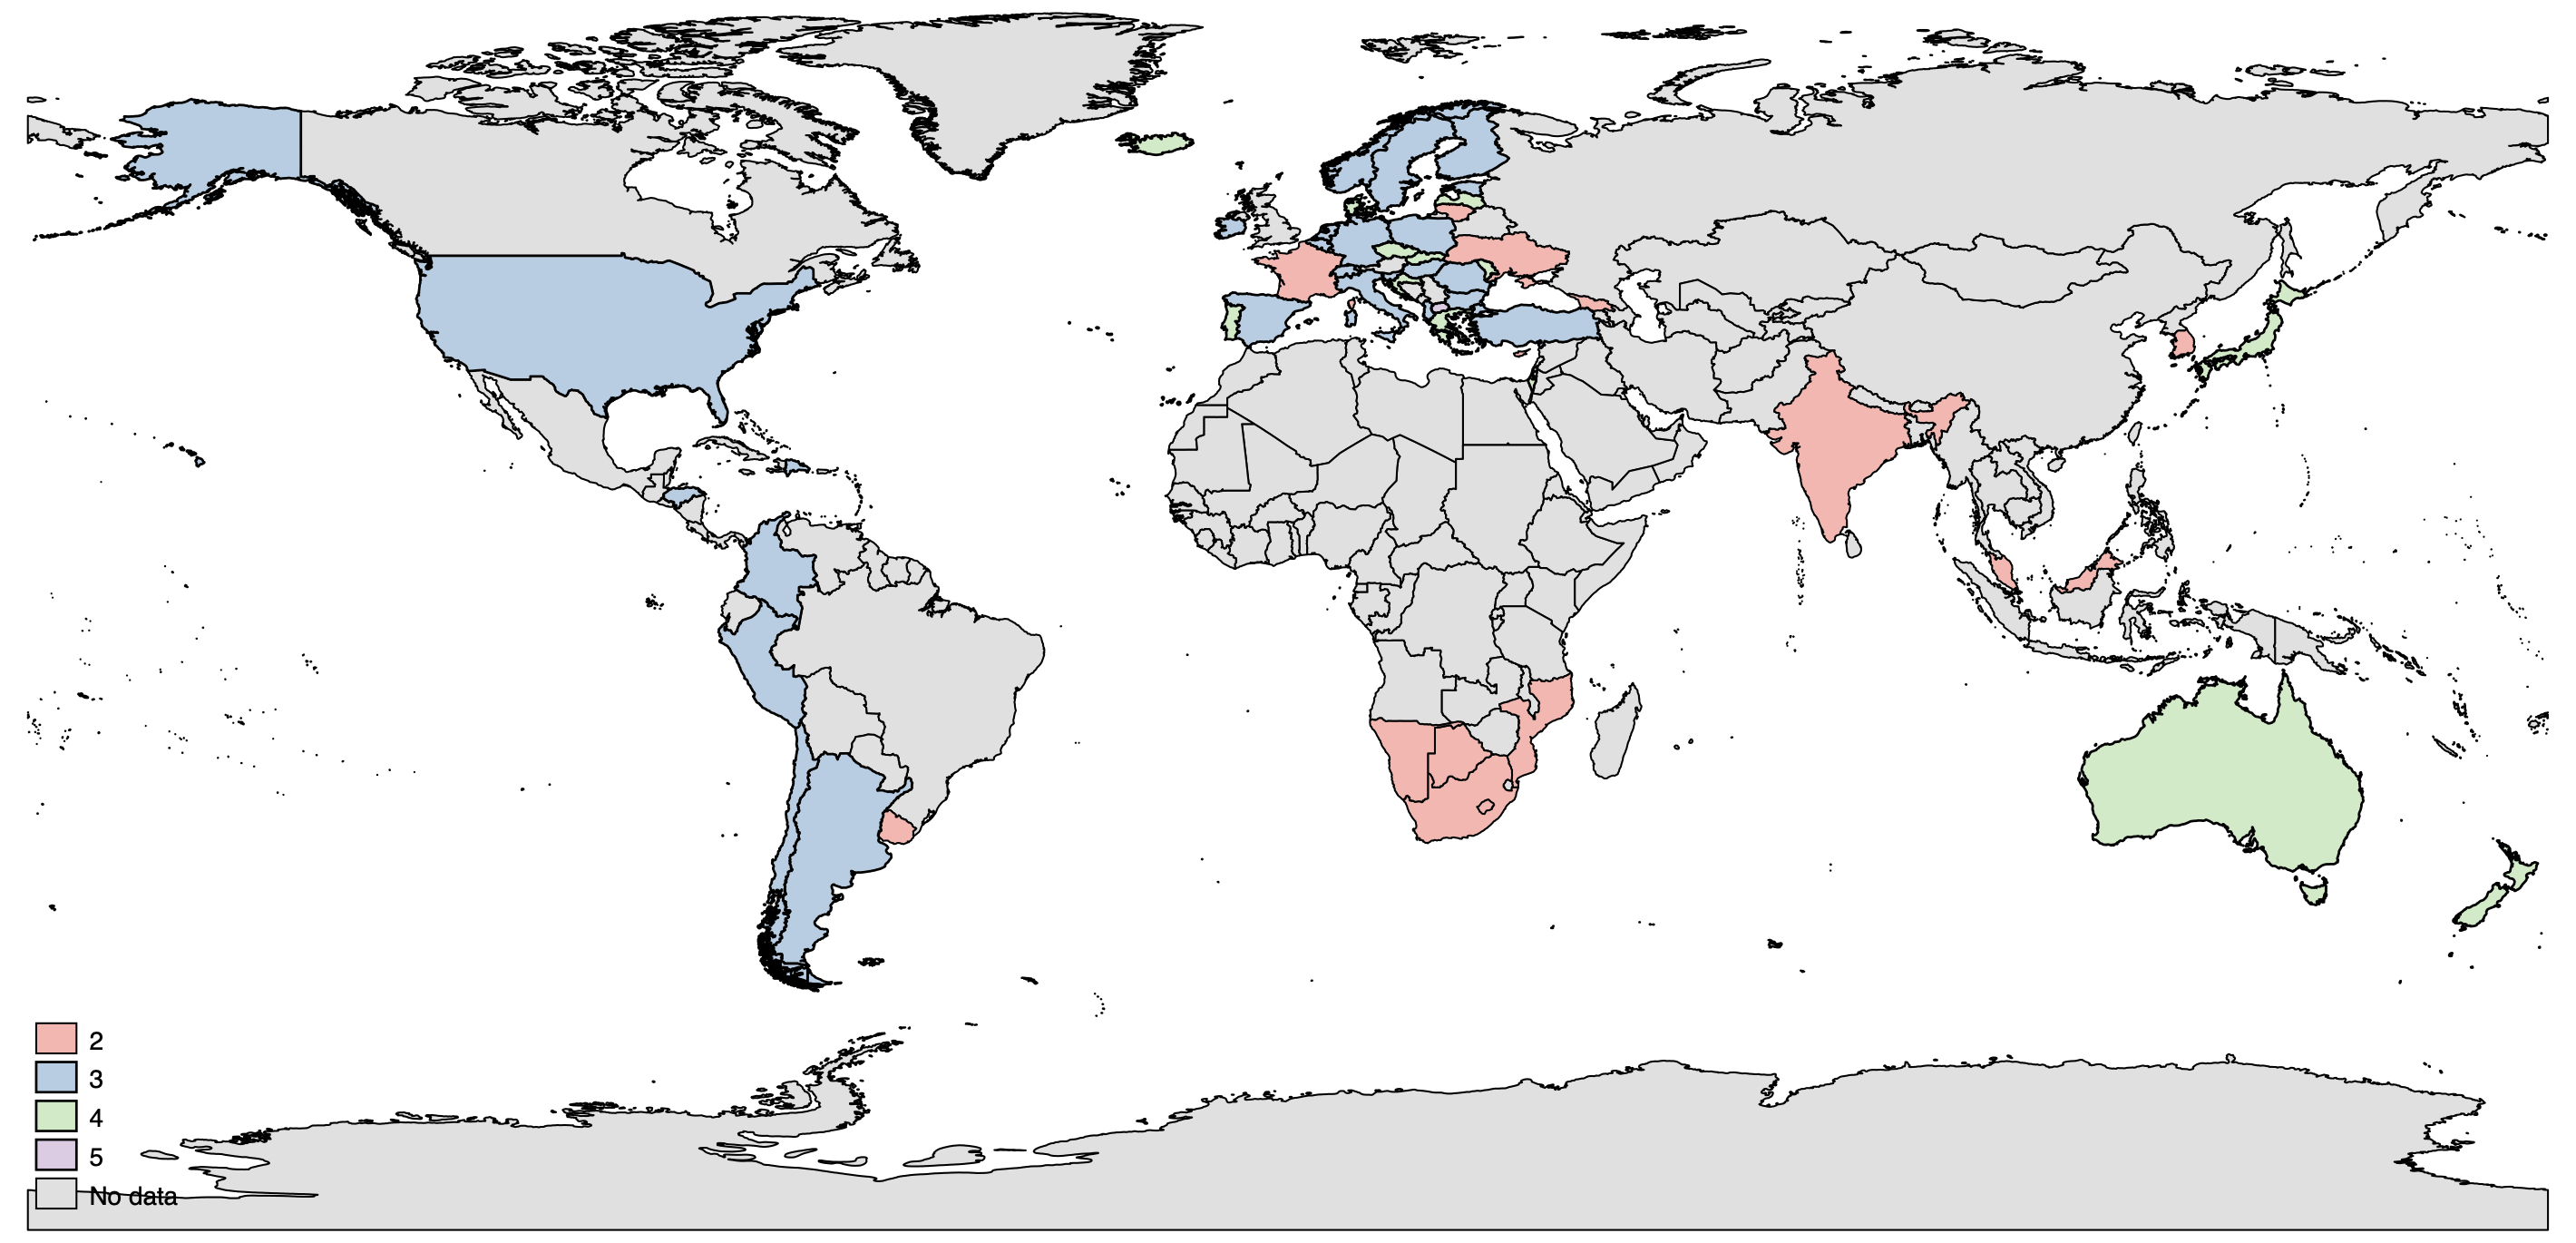
\includegraphics[scale=0.45]{../output/plots/map1.png}
	\caption{Distribution of elections across countries for Sample A.}
	\label{map1}
\end{figure}

\begin{figure}[th]
	\centering
	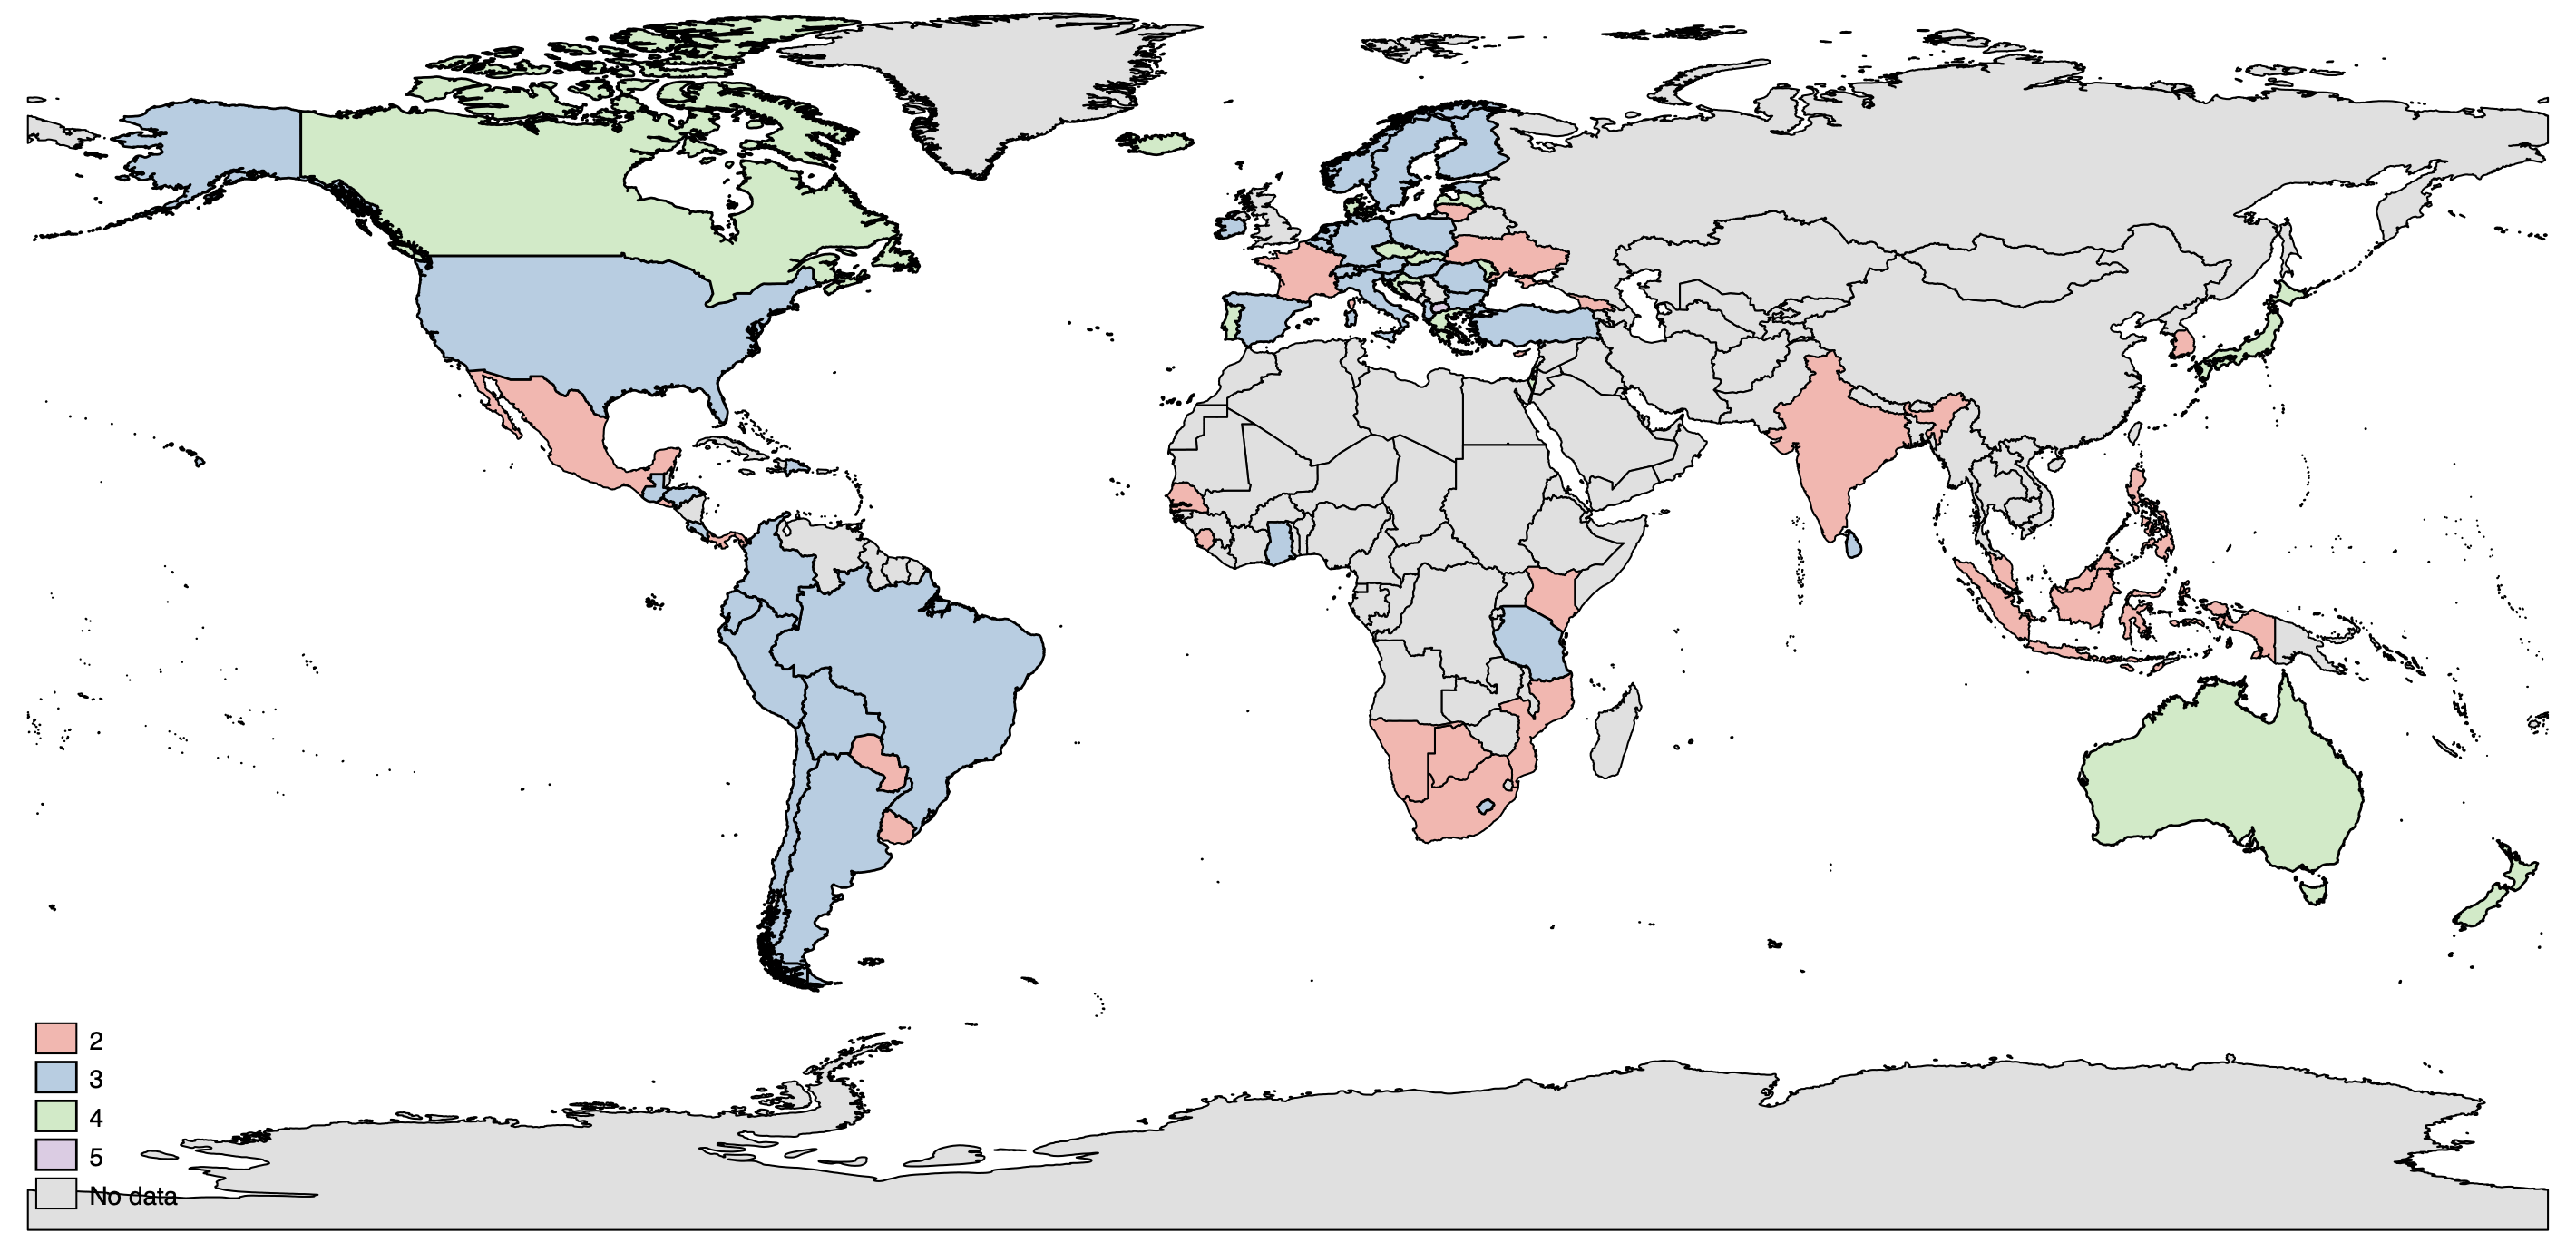
\includegraphics[scale=0.45]{../output/plots/map2.png}
	\caption{Distribution of elections across countries for Sample B.}
	\label{map2}
\end{figure}
\end{landscape}

\clearpage
\begin{figure}[th]
	\centering
	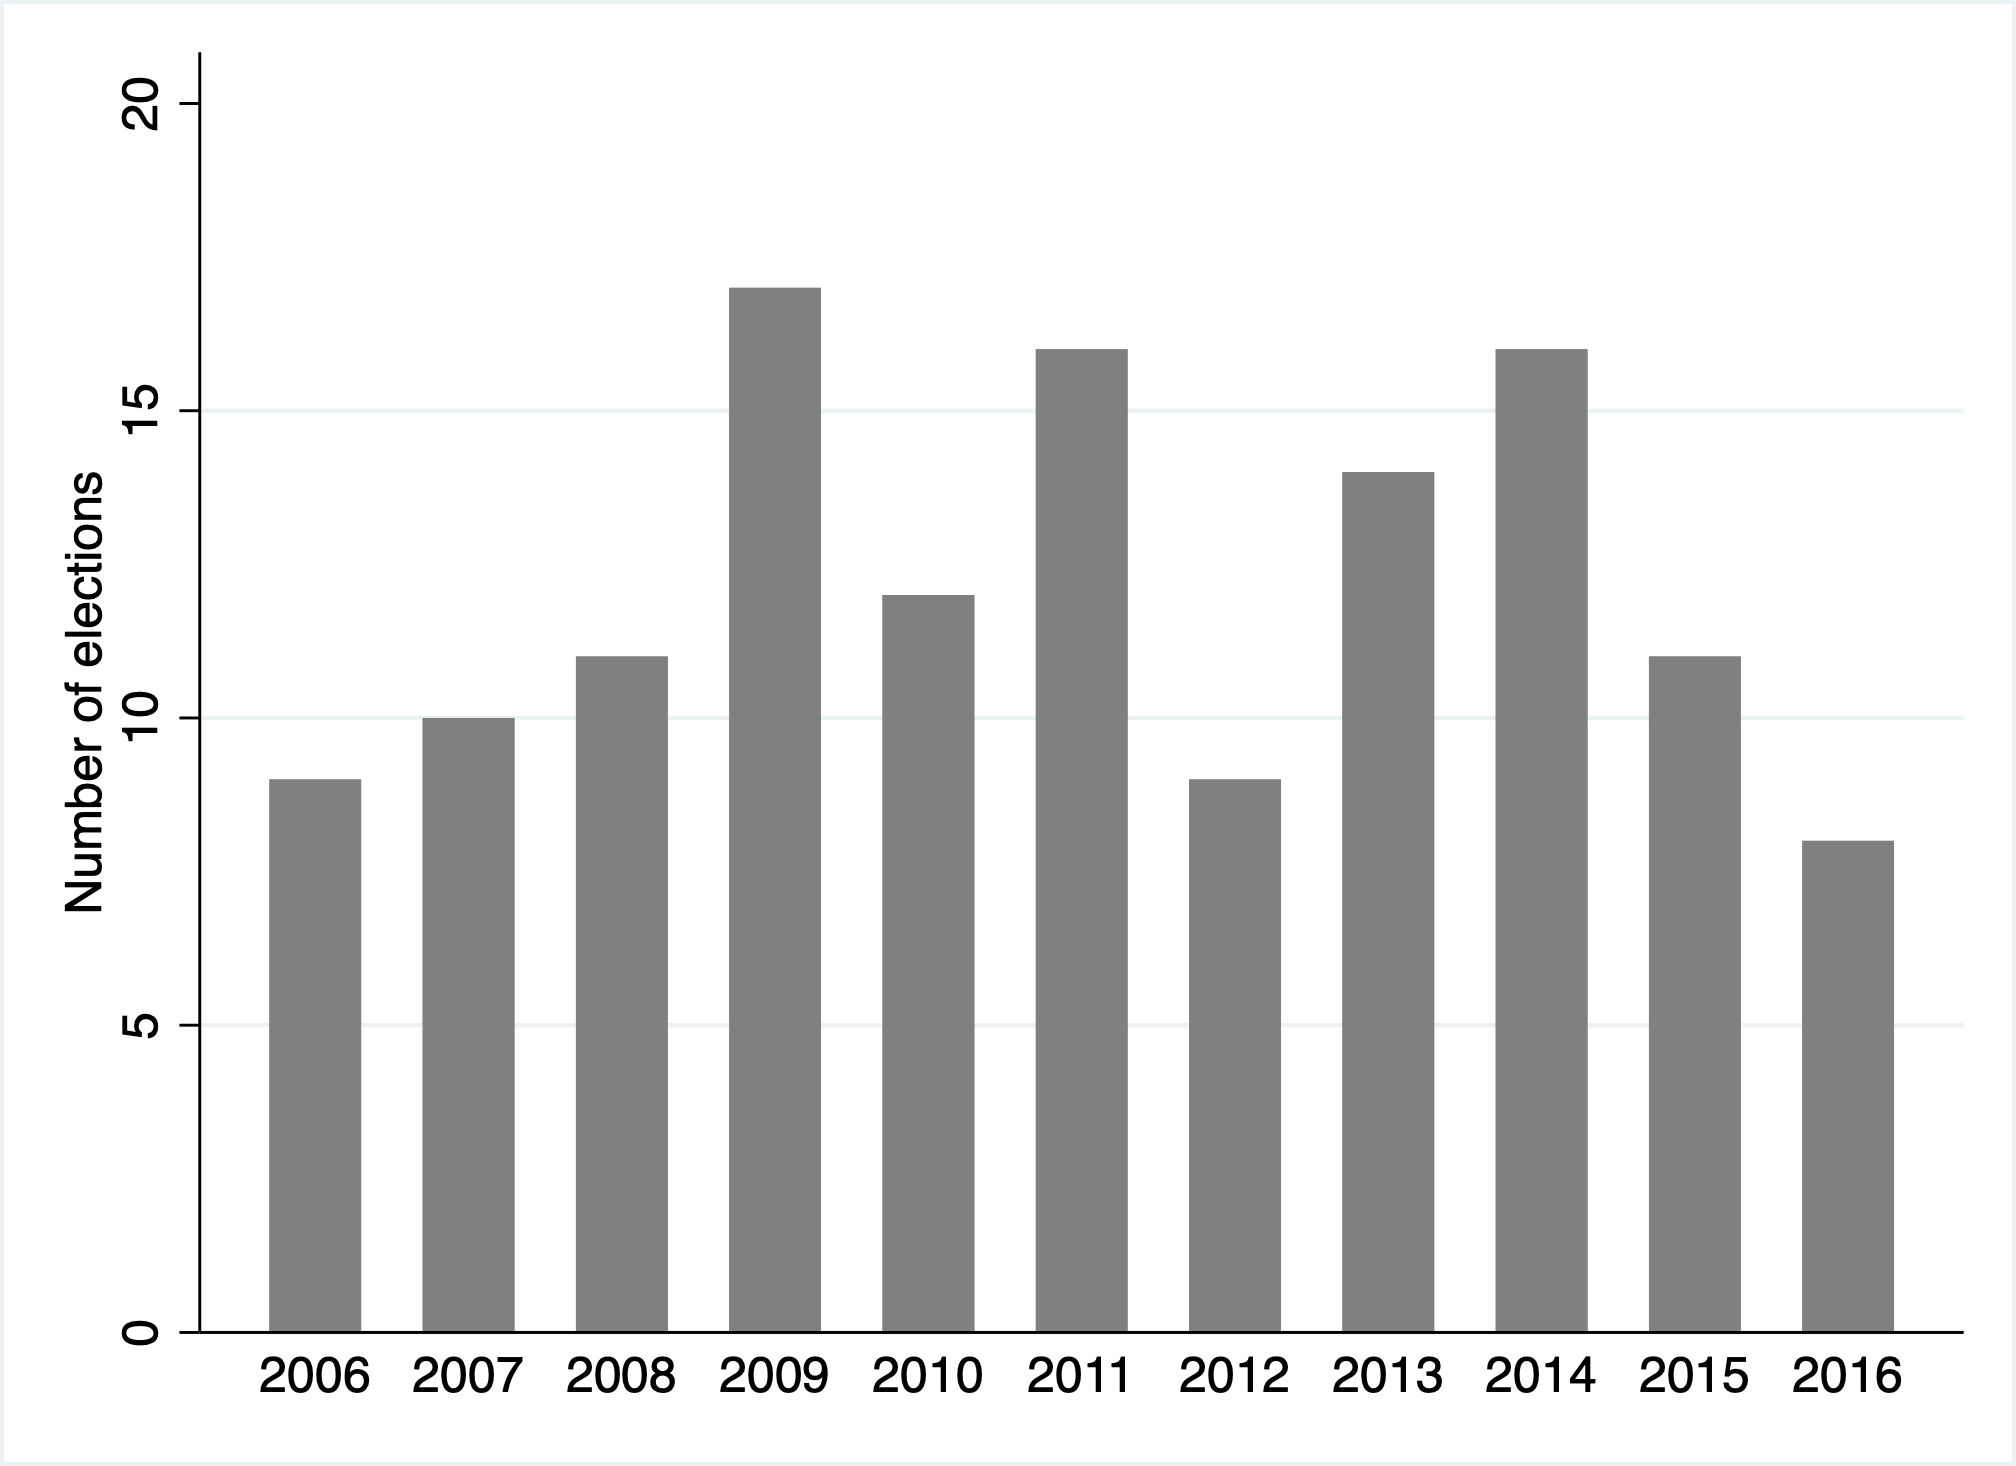
\includegraphics[scale=0.4]{../output/plots/elec_freq.png}
	\caption{Distribution of elections across time for Sample A.}
	\label{bar1}
\end{figure}

\begin{figure}[h!]
	\centering
	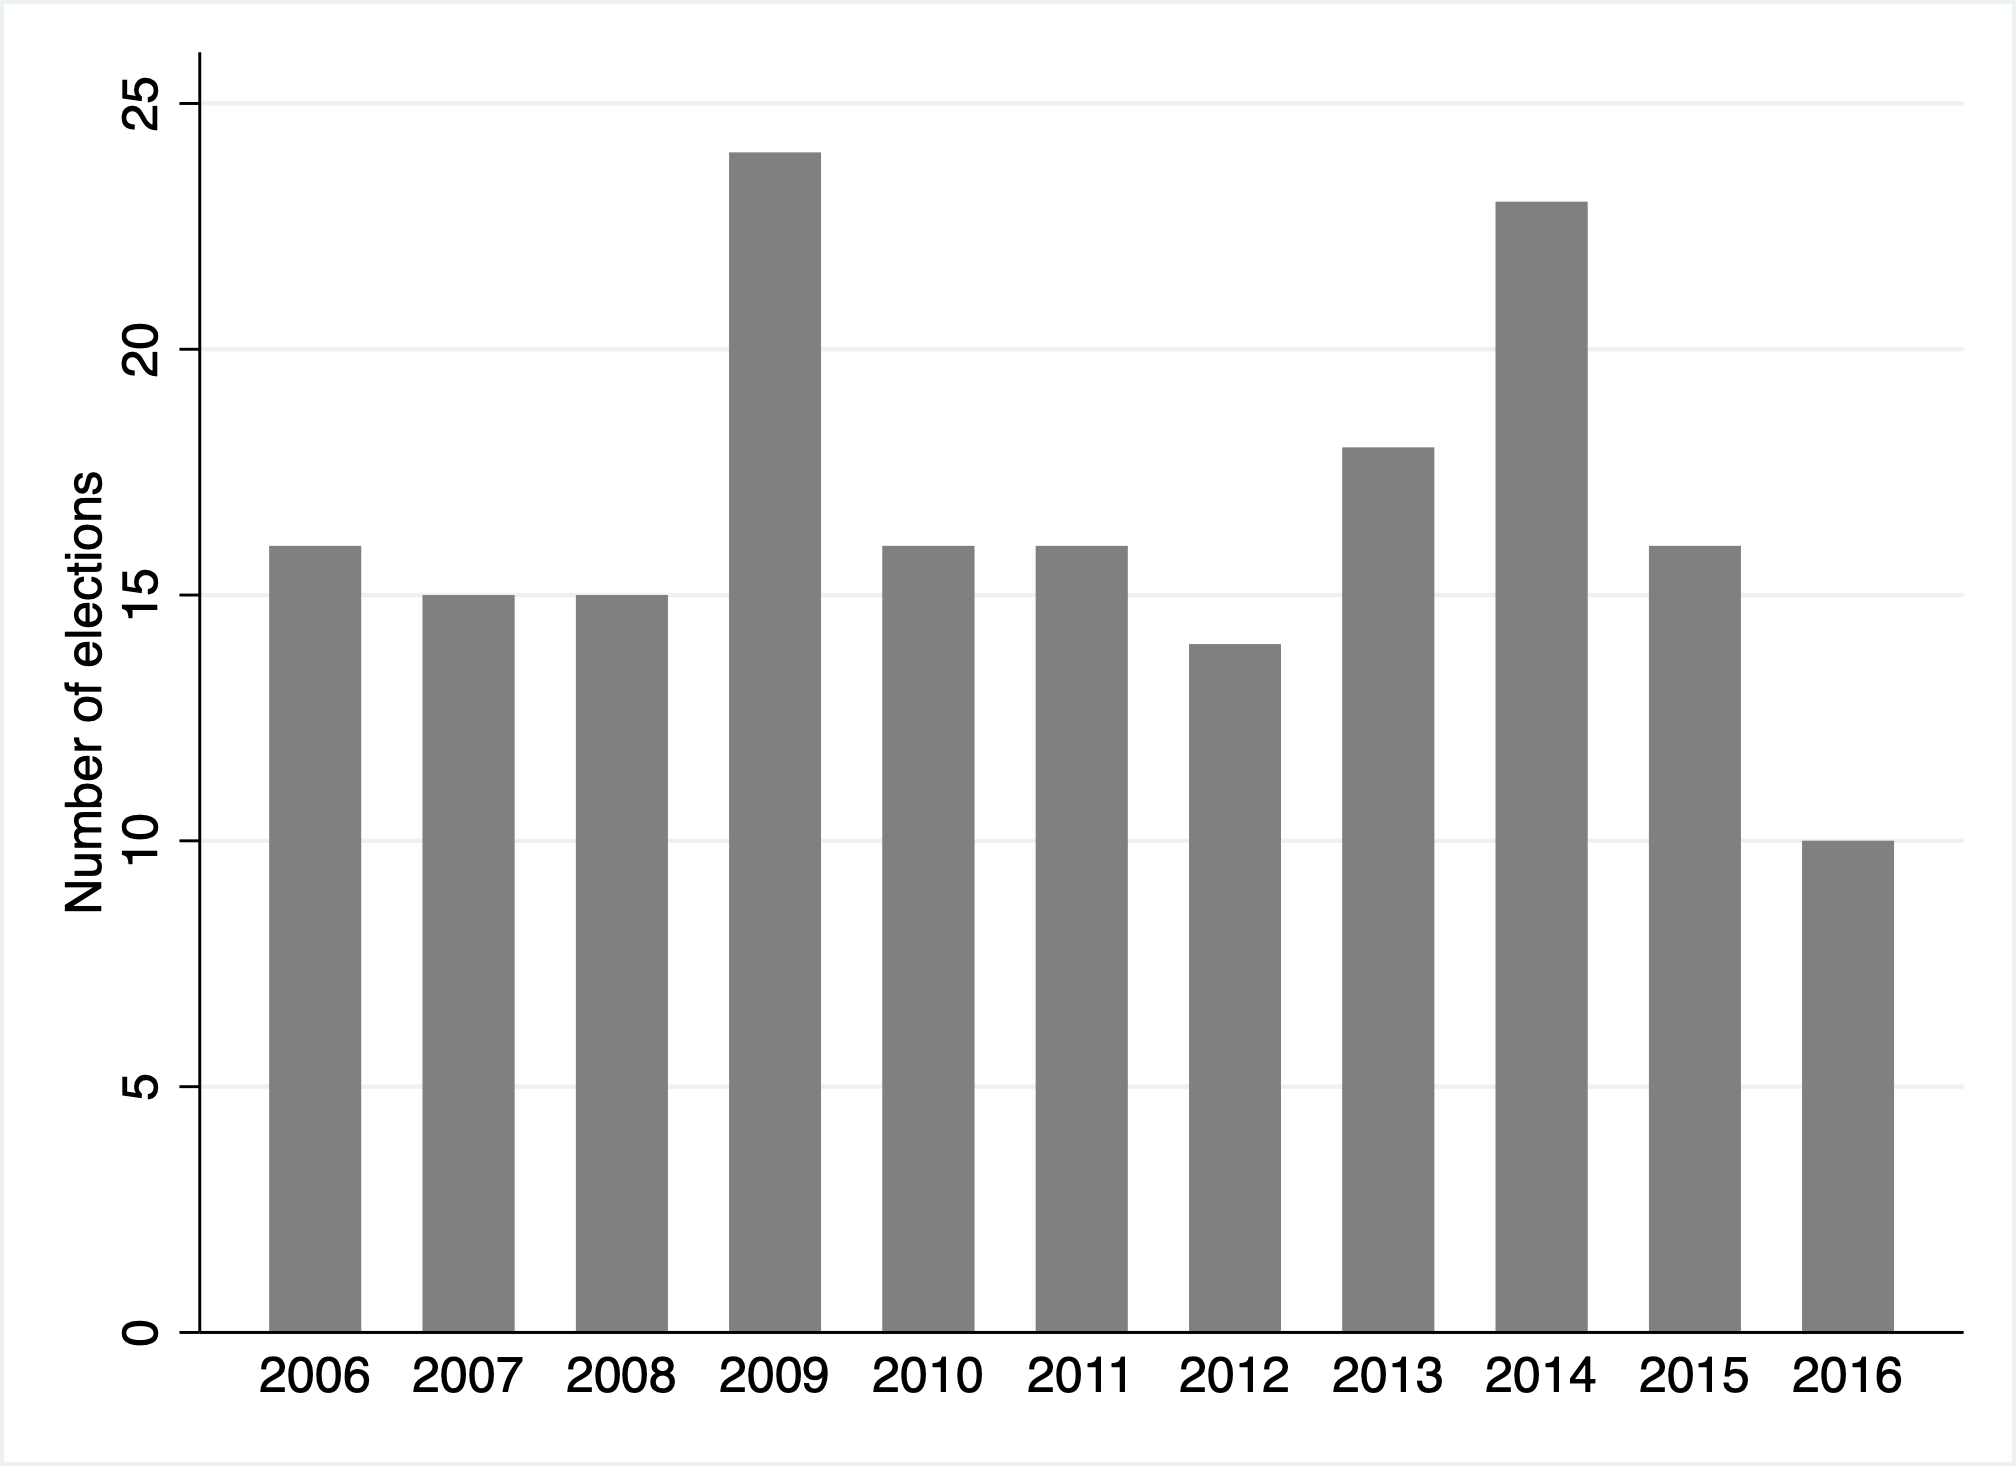
\includegraphics[scale=0.4]{../output/plots/elec_freq2.png}
	\caption{Distribution of elections across time for Sample B.}
	\label{bar2}
\end{figure}

\clearpage

\end{document}
